\chapter{Formulazione Teorica e Framework Metodologico}
\label{ch:metodologia}

Il presente capitolo definisce l'impalcatura teorica e il framework metodologico alla base dell'intera indagine sperimentale, fornendo gli strumenti formali necessari per la modellazione, l'analisi e l'adattamento dei sistemi di \textit{Network Intrusion Detection} (NIDS) in contesti operativi eterogenei. L'obiettivo primario risiede nell'instaurazione di un paradigma valutativo rigoroso, strutturalmente svincolato dalle specificità implementative dei singoli dataset, che consenta di quantificare oggettivamente i fenomeni di traslazione di dominio (\textit{domain shift}) e di validare le performance di generalizzazione isolando i reali contributi algoritmici dalla varianza stocastica.

La trattazione si articola secondo una progressione logica suddivisa in quattro sezioni principali:
\begin{itemize}
    \item La \textbf{Sezione~\ref{sec:modello_sistema}} formalizza il modello astratto del sistema, definendo rigorosamente gli spazi vettoriali di rappresentazione, gli operatori di proiezione per l'armonizzazione delle \textit{feature} e le regole architetturali di partizionamento dei domini.
    \item La \textbf{Sezione~\ref{sec:tassonomia_modelli}} delinea la tassonomia delle architetture di classificazione adottate e le relative strategie di \textit{transfer learning}, uniformando le metriche di confronto mediante una formulazione omogenea basata sulla stima della probabilità a posteriori.
    \item La \textbf{Sezione~\ref{sec:framework_adattamento}} stabilisce il protocollo valutativo per la stabilità statistica, affrontando la gestione dell'incertezza stocastica tramite valutazione \textit{multi-seed} e definendo gli indici morfologici di granularità dello spazio decisionale.
    \item Infine, la \textbf{Sezione~\ref{sec:framework_analitico}} completa l'architettura metodologica descrivendo l'apparato diagnostico e di \textit{explainability}, integrando strumenti di stima di densità e metriche di rilevanza fondate sulla teoria dei giochi cooperativi per la caratterizzazione e l'interpretazione causale delle divergenze distributive.
\end{itemize}

\section{Modello del Sistema e Spazi di Rappresentazione}
\label{sec:modello_sistema}

La presente sezione formalizza l'impalcatura teorica e matematica del framework analitico, definendo in modo rigoroso gli spazi vettoriali di rappresentazione e le distribuzioni di probabilità necessarie per modellare i fenomeni di transizione cross-dominio nei sistemi NIDS. 
L'obiettivo è stabilire un modello astratto, indipendente dalle peculiarità di implementazione dei singoli dataset, in grado di garantire il rigore metodologico, la comparabilità delle metriche e l'assenza di contaminazione informativa.

Questa formalizzazione prosegue direttamente la disamina svolta nel Capitolo~\ref{ch:bck_rltd_wrks}, traducendo in termini matematici e procedurali le criticità del confronto tra segmenti terrestri e spaziali e le esigenze di adattamento dei NIDS delineate nel contesto di riferimento.

A tal fine, la trattazione introduce preliminarmente la formalizzazione dei domini di origine e destinazione, delineando la semantica a doppia etichettatura $(Y, A)$, le regole di partizionamento preventivo anti-\textit{data leakage} e il vincolo di proporzionamento parametrico $\rho$ alla base delle cinque categorie astratte di benchmark, native e ibride, istanziabili dal framework. 
Successivamente, viene definito l'operatore di proiezione $\boldsymbol{\psi}_k$, specifico per ciascun dominio $k \in \{S, T\}$, che mappa le caratteristiche grezze eterogenee nello spazio delle \textit{feature} condiviso $\mathcal{X}$, esplicitando i criteri concettuali di filtraggio e armonizzazione degli attributi. 
La trattazione si conclude motivando, sulla base della proprietà di invarianza rispetto a trasformazioni monotoniche propria dei classificatori a partizionamento ricorsivo, l'omissione della fase esplicita di scalatura dalla definizione dello spazio delle \textit{feature}.

Per facilitare la lettura della trattazione successiva, i principali simboli e costrutti matematici adottati sono sintetizzati nella Tabella~\ref{tab:notazione_matematica}.

\begin{table}[H]
    \centering
    \caption{Sintesi della notazione matematica e dei simboli del framework.}
    \label{tab:notazione_matematica}
    \small
    \renewcommand{\arraystretch}{1.3}
    \begin{tabularx}{\textwidth}{@{} >{\raggedright\arraybackslash}p{3cm} >{\raggedright\arraybackslash}X @{} }
    \toprule
    \textbf{Simbolo} & \textbf{Descrizione e Significato Concettuale} \\
    \midrule
    $\mathcal{D} = (\mathcal{X}, P(\mathbf{x}))$ &
    Dominio di traffico (spazio delle \textit{feature} e distribuzione marginale) \\

    $\mathcal{X} \subseteq \mathbb{R}^d$ &
    Spazio delle caratteristiche $d$-dimensionale omogeneizzato \\

    $\mathbf{x} = (x_1, \dots, x_d)^\top$ &
    Vettore delle \textit{feature} del singolo flusso di rete \\

    $\mathcal{Y} = \{0,1\}$ &
    Spazio discreto delle etichette primarie ($0$: Normal, $1$: Malevolo) \\

    $A \in \mathcal{A}$ &
    Variabile descrittiva per la specifica famiglia di attacco (definita per $Y=1$) \\

    $\mathcal{A}_S, \mathcal{A}_T$ &
    Insiemi delle tipologie di minaccia presenti nei domini sorgente e target \\

    $\mathcal{D}_S, \mathcal{D}_T$ &
    Dominio Terrestre Sorgente e Domini Target di Destinazione \\

    $\mathcal{D}_k^{(train)}, \mathcal{D}_k^{(test)}$ &
    Partizioni disgiunte di addestramento e test per il generico dominio $k$ \\

    $\boldsymbol{\psi}_k(\cdot)$ &
    Operatore di proiezione e combinazione dalle \textit{feature} grezze allo spazio $\mathcal{X}$, specifico per il dominio $k \in \{S,T\}$ \\

    $N(\cdot)$ &
    Operatore di cardinalità (numero di campioni estratti) \\
    \bottomrule
    \end{tabularx}
\end{table}

\subsection{Formalizzazione dei Domini e Composizione Asimmetrica del Traffico}
\label{subsec:composizione_domini}

Il framework analitico richiede la definizione rigorosa degli spazi di rappresentazione vettoriale e delle distribuzioni di probabilità associate ai diversi contesti di rete considerati. Si definisce un dominio $\mathcal{D}$ come la coppia $(\mathcal{X}, P(\mathbf{x}))$, dove $\mathcal{X} \subseteq \mathbb{R}^d$ rappresenta lo spazio delle \textit{feature} $d$-dimensionale condiviso e $P(\mathbf{x})$ la distribuzione di probabilità marginale definita sul vettore delle caratteristiche $\mathbf{x} = (x_1, x_2, \dots, x_d)^\top \in \mathcal{X}$.

Associato a ciascun dominio, la semantica del traffico è modellata tramite una doppia etichettatura. Lo spazio discreto primario $\mathcal{Y} = \{0,1\}$ stabilisce la natura del flusso, dove $Y = 0$ indica il traffico nominale (\textit{Normal}) e $Y = 1$ identifica genericamente un vettore malevolo. In aggiunta, si definisce un'ulteriore variabile descrittiva $A \in \mathcal{A}$ che specifica il nome della classe, garantendo una caratterizzazione puntuale sia per la componente benevola ($Y = 0$), per la quale $A$ assume tipicamente un unico valore costante (\textit{Normal}), sia per le diverse famiglie di attacco ($Y = 1$), per le quali $A$ è genuinamente multi-valore.

\subsubsection{Caratterizzazione Astratta dei Domini e Tassonomia delle Classi}
\label{subsubsec:caratterizzazione_domini}
Il framework analitico modella il fenomeno di transizione cross-dominio a partire da due macro-distribuzioni di partenza distinte:
\begin{enumerate}
    \item \textbf{Dominio di Riferimento ($\mathcal{D}_S$):} rappresenta l'ambiente stazionario di origine, contenente sia istanze di traffico nominale ($Y = 0, A \in \mathcal{A}_S$) sia flussi malevoli ($Y = 1, A \in \mathcal{A}_S$). Per eliminare le componenti ad elevata sparsità ed esigua rappresentatività statistica, si applica una procedura di rimozione delle classi minoritarie (\textit{minority removal}) sull'insieme $\mathcal{A}_S$, garantendo una caratterizzazione stabile del baseline di superficie.
    \item \textbf{Domini di Destinazione ($\mathcal{D}_T$):} rappresentano i contesti soggetti a variazioni trasmissive o canali eterogenei, composti esclusivamente da vettori di traffico malevolo ($Y = 1, A \in \mathcal{A}_T$). Tali domini vengono strutturati applicando, laddove necessario, un raggruppamento delle classi minoritarie (\textit{minority merge}) per accorpare famiglie d'attacco semanticamente affini e preservare la significatività campionaria.
\end{enumerate}

\subsubsection{Isolamento Preventivo delle Partizioni e Politiche Anti-Data Leakage}
\label{subsubsec:isolamento_partizioni}
Per garantire il rigore metodologico ed evitare fenomeni di contaminazione informativa tra la fase di addestramento e quella di valutazione (\textit{data leakage})\footnote{L'esecuzione dello split a monte di qualsiasi fusione previene che campioni identici della classe nominale, riutilizzati per benchmark diversi, compaiano simultaneamente negli insiemi di addestramento e di test.}, la partizione di ciascun dominio primario $\mathcal{D}_k$ nei sotto-insiemi di addestramento ($\mathcal{D}_k^{(train)}$) e di verifica ($\mathcal{D}_k^{(test)}$) viene definita a monte di qualsiasi aggregazione o composizione dei benchmark derivati\footnote{Dal punto di vista metodologico, tale partizionamento e la successiva ricomposizione dei vettori vengono eseguiti prima di qualsiasi composizione dei benchmark, evitando la creazione di dataset intermedi.}. In tutte le configurazioni sperimentali viene adottata una suddivisione stocastica stratificata con proporzione fissa:
\begin{equation}
    \mathcal{D}_k = \mathcal{D}_k^{(train)} \cup \mathcal{D}_k^{(test)}, \quad \text{con } \mathcal{D}_k^{(train)} \cap \mathcal{D}_k^{(test)} = \emptyset
    \label{eq:split_train_test}
\end{equation}
garantendo la totale indipendenza strutturale dei vettori impiegati per l'inferenza.

\subsubsection{Sintesi dei Benchmark e Vincoli di Proporzionamento Riconfigurato}
\label{subsubsec:sintesi_benchmark}
Sia per le configurazioni generate internamente al dominio sorgente sia per i benchmark ibridi ricomposti cross-dominio (necessari per l'assenza di traffico nominale etichettato nei contesti di destinazione), il framework applica una politica di proporzionamento controllato.

Per rispecchiare le condizioni realistiche di rete e prevenire uno sbilanciamento artificiale dei classificatori\footnote{Nei sistemi NIDS reali, il traffico lecito costituisce la stragrande maggioranza del volume di rete. La parametrizzazione del rapporto emula tale asimmetria mantenendo una densità di attacchi sufficiente a garantire la stabilità statistica delle metriche.}, il framework impone un vincolo di proporzionamento parametrico $\rho$ tra la componente benevola e la componente malevola complessiva:
\begin{equation}
    \frac{N(Y = 0)}{\sum_{a \in \mathcal{A}_m} N(Y = 1, A = a)} = \rho
    \label{eq:rho_constraint}
\end{equation}
Tale vincolo definisce in modo esplicito l'asimmetria volumetrica tra il traffico nominale ($Y = 0$) e il traffico malevolo ($Y = 1$). Dove $N(\cdot)$ indica la cardinalità dei campioni estratti, $\mathcal{A}_m$ rappresenta l'insieme delle specifiche famiglie di attacco incluse nella configurazione e $\rho \in \mathbb{R}^+$ costituisce il fattore di asimmetria volumetrica prescritto dal protocollo metodologico.

A livello di estrazione, come regola generale si adotta il campionamento senza reinserimento (\textit{without replacement}), precludendo la duplicazione sintetica delle istanze. Qualora, a seguito dell'applicazione del rapporto $\rho$, una delle due classi $Y \in \{0, 1\}$ non disponga di una quantità di dati sufficiente a raggiungere il volume teorico prefissato, il framework rifiuta l'uso del \textit{replacing}. In tale evenienza, il dimensionamento complessivo del benchmark si ridimensiona ancorandosi alla classe minoritaria (ovvero quella con minore disponibilità di campioni): l'estrazione per l'altra classe viene riproporzionata di conseguenza per soddisfare il rapporto $\rho$, accettando la potenziale perdita o il mancato utilizzo di una quota di campioni della classe maggioritaria pur di preservare l'unicità e l'integrità statistica delle osservazioni.

Nei benchmark di tipo aggregato (sia sorgenti che ibridi), la composizione interna del sottoinsieme malevolo non adotta l'equiprobabilità artificiale tra le classi d'attacco. Si preserva invece la distribuzione naturale \textit{a priori} $P(A = a \mid Y = 1)$ caratteristica dei domini di origine, evitando alterazioni sintetiche e mantenendo la fedeltà alle frequenze di occorrenza reali delle minacce.

L'intero processo di isolamento procedurale e ricomposizione dei benchmark è schematizzato nella Figura~\ref{fig:flusso_benchmark}.

\begin{figure}[H]
    \centering
    \resizebox{0.9\textwidth}{!}{%
    \begin{tikzpicture}[
        >={Stealth[length=2mm, width=1.4mm]},
        domnode/.style={
            rectangle, draw=black, fill=gray!10, thick,
            align=center, rounded corners=2pt, inner sep=5pt
        },
        process/.style={
            rectangle, draw=black, fill=white, thick, dashed,
            align=center, inner sep=5pt
        },
        cat/.style={
            rectangle, draw=black, fill=gray!30, thick,
            align=center, rounded corners=2pt, inner sep=5pt
        },
        line/.style={draw=black, thick, ->},
    ]

        % RIGA 1: Domini Primari
        \node [domnode] (source) at (-4, 9.2) {
            \textbf{Dominio Sorgente $\mathcal{D}_S$}\\
            $P_S(\mathbf{x}\mid Y{=}0, A\in\mathcal{A}_S) \cup P_S(\mathbf{x}\mid Y{=}1, A\in\mathcal{A}_S)$
        };
        \node [domnode] (target) at (4, 9.2) {
            \textbf{Domini Target $\mathcal{D}_T$}\\
            $P_T(\mathbf{x}\mid Y{=}1, A\in\mathcal{A}_T)$
        };

        % RIGA 2: Allineamento e Split Logico
        \node [process] (split_s) at (-4, 7) {
            \textbf{Allineamento di $\mathcal{X}$ (\S\,\ref{subsec:allineamento_feature}) e}\\
            \textbf{Isolamento Logico} (Train/Test)
        };
        \node [process] (split_t) at (4, 7) {
            \textbf{Allineamento di $\mathcal{X}$ (\S\,\ref{subsec:allineamento_feature}) e}\\
            \textbf{Isolamento Logico} (Train/Test)
        };

        % RIGA 3: Sintesi Logica (Aggiornato con vincolo senza reinserimento)
        \node [process] (synth) at (0, 3.9) {
            \textbf{Sintesi Logica}\\
            $\mathcal{D}_S^{(train)} \cup \mathcal{D}_T^{(train)}$ \quad e, \textit{separatamente}, \quad $\mathcal{D}_S^{(test)} \cup \mathcal{D}_T^{(test)}$\\
            \textit{Asimmetria volumetrica: Ratio $\rho$ (Senza Reinserimento)}\\
            \textit{Prior naturali in aggregato}
        };

        % RIGA 4: Categorie Risultanti
        \node [cat] (categories) at (0, 0) {
            \textbf{Tipologie di Benchmark Istanziati a Runtime}\\
            Nativi Sorgente (Aggregati e Biclasse)\\
            Ibridi (Aggregati e Biclasse)\\
            Iniezione (Aggregato)
        };

        % CONNESSIONI
        \draw [line] (source) -- (split_s.north);
        \draw [line] (target) -- (split_t.north);

        \draw [line] (split_s.south) -- ++(0,-0.5) -| ($(synth.north)+(-1,0)$);
        \draw [line] (split_t.south) -- ++(0,-0.5) -| ($(synth.north)+(1,0)$);

        \draw [line] (synth.south) -- (categories.north);

    \end{tikzpicture}
    }
    \caption{Pipeline logica astratta: allineamento dello spazio delle feature $\mathcal{X}$, isolamento preventivo Train/Test anti-\textit{data leakage}, sintesi parametrica con ratio $\rho$ senza reinserimento (con ancoraggio alla classe minoritaria) e istanziazione logica dei benchmark. I blocchi tratteggiati indicano le elaborazioni logiche, mentre i blocchi a linea continua rappresentano gli insiemi di dati e le categorie di output.}
    \label{fig:flusso_benchmark}
\end{figure}

\subsubsection{Tassonomia Astratta delle Configurazioni Sperimentali}
\label{subsubsec:tassonomia_configurazioni}
L'applicazione sistematica delle regole metodologiche descritte porta alla generazione dinamica di cinque categorie funzionali di benchmark. Ognuna di queste configurazioni viene istanziata logicamente rispettando il preventivo isolamento logico delle partizioni di train e test e imponendo il vincolo di proporzionamento parametrico $\rho$ tra traffico benevolo e malevolo:
\begin{enumerate}
    \item \textbf{Set Nativo Sorgente Aggregato:} composto dalla baseline nominale $Y=0$ di $\mathcal{D}_S$ unita alla totalità delle famiglie di attacco sorgenti $A \in \mathcal{A}_S$ (a valle della procedura di \textit{minority removal}), preservando la distribuzione naturale a priori $P(A = a \mid Y = 1)$ caratteristica del dominio di origine.
    \item \textbf{Set Nativi Sorgente Biclasse:} formati dall'unione della classe nominale $Y=0$ con una singola famiglia di attacco $A = a \in \mathcal{A}_S$ isolata all'interno del dominio sorgente.
    \item \textbf{Set Ibridi Aggregati:} composti dalla classe nominale $Y=0$ del dominio sorgente unita alla totalità delle minacce dei domini di destinazione $A \in \mathcal{A}_T$ (strutturate tramite \textit{minority merge}), preservando le frequenze \textit{a priori} originali del dominio target.
    \item \textbf{Set Ibridi Biclasse:} formati dalla combinazione della classe nominale $Y=0$ sorgente con le singole famiglie d'attacco $A = a \in \mathcal{A}_T$ isolate all'interno dei domini target.
    \item \textbf{Set di Iniezione di Riferimento:} progettato in conformità agli standard di letteratura~\cite{azar2023}, mantiene l'intera distribuzione nativa del dominio sorgente (sia il traffico nominale che l'aggregato malevolo di $\mathcal{D}_S$) integrandola con un'iniezione sparsa e controllata di vettori d'attacco provenienti dai domini target $\mathcal{D}_T$.
\end{enumerate}

I dettagli analitici di composizione per ciascuna delle cinque categorie, opportunamente suddivisi per natura del traffico, sono riassunti nella Tabella~\ref{tab:tassonomia_benchmark}.

\begin{table}[H]
    \centering
    \caption{Tassonomia astratta delle cinque categorie di benchmark sperimentali istanziate dinamicamente.}
    \label{tab:tassonomia_benchmark}
    \small
    \renewcommand{\arraystretch}{1.3}
    \begin{tabularx}{\textwidth}{@{} >{\raggedright\arraybackslash}p{3.5cm} >{\raggedright\arraybackslash}X >{\raggedright\arraybackslash}X @{} }
    \toprule
    \textbf{Categoria Benchmark} & \textbf{Componente Benevola ($Y=0$)} & \textbf{Componente Malevola ($Y = 1$)} \\
    \midrule
    \textbf{Set Nativo Sorgente Aggregato} &
    Baseline nativa $P_S(\mathbf{x} \mid Y=0, A \in \mathcal{A}_S)$ &
    Tutte le minacce sorgente $P_S(\mathbf{x} \mid Y=1, A \in \mathcal{A}_S)$ con distribuzioni \textit{a priori} naturali. \\

    \textbf{Set Nativo Sorgente Biclasse} &
    Baseline nativa $P_S(\mathbf{x} \mid Y=0, A \in \mathcal{A}_S)$ &
    Singola minaccia sorgente $P_S(\mathbf{x} \mid Y=1, A = a)$ isolata ($a \in \mathcal{A}_S$). \\

    \textbf{Set Ibrido Aggregato} &
    Baseline nativa $P_S(\mathbf{x} \mid Y=0, A \in \mathcal{A}_S)$ &
    Tutte le minacce target $P_T(\mathbf{x} \mid Y=1, A \in \mathcal{A}_T)$ con distribuzioni \textit{a priori} naturali. \\

    \textbf{Set Ibrido Biclasse} &
    Baseline nativa $P_S(\mathbf{x} \mid Y=0, A \in \mathcal{A}_S)$ &
    Singola minaccia target $P_T(\mathbf{x} \mid Y=1, A = a)$ isolata ($a \in \mathcal{A}_T$). \\

    \textbf{Set di Iniezione di Riferimento} &
    Baseline nativa $P_S(\mathbf{x} \mid Y=0, A \in \mathcal{A}_S)$ &
    Minacce sorgente in aggregato $P_S(\mathbf{x} \mid Y=1, A \in \mathcal{A}_S)$ \\
    & & \textbf{+} iniezione altamente sparsa da $\mathcal{D}_T$ ($A \in \mathcal{A}_T$). \\
    \bottomrule
    \end{tabularx}
\end{table}

\subsection{Allineamento dello Spazio delle Feature e Preprocessing Astratto}
\label{subsec:allineamento_feature}

La disomogeneità strutturale tra le sonde di rilevamento e i formati di tracciamento adottati nei diversi ambienti di rete comporta un'asimmetria nativa negli spazi delle caratteristiche grezze. Per consentire la comparabilità cross-dominio, il framework definisce una procedura astratta di riallineamento spaziale e un impianto di trasformazione che mappa osservazioni eterogenee in uno spazio vettoriale comune, preservando la semantica trasmissiva e ottimizzando l'efficienza concettuale. L'intero flusso di mappatura è sintetizzato in Figura~\ref{fig:allineamento_feature}.

\subsubsection{Mappatura e Omogeneizzazione dello Spazio Vettoriale}
\label{subsubsec:mappatura_feature}
Siano $\mathcal{X}_S^{(grezzo)} \subseteq \mathbb{R}^{d_S}$ e $\mathcal{X}_T^{(grezzo)} \subseteq \mathbb{R}^{d_T}$ gli spazi delle caratteristiche grezze associati rispettivamente al dominio sorgente e ai domini di destinazione. Per superare le differenze nomenclaturali, metriche e strutturali tra le $d_S$ e $d_T$ variabili native, si definisce, per ciascun dominio $k \in \{S, T\}$, un operatore di trasformazione e combinazione funzionale $\boldsymbol{\psi}_k: \mathbb{R}^{d_k} \rightarrow \mathbb{R}^d$ tale per cui\footnote{La dimensione ridotta $d$ costituisce una costante uniforme per l'intero framework.}:
\begin{equation}
    \mathbf{x}_k = \boldsymbol{\psi}_k(\mathbf{x}_k^{(grezzo)}) = \left( \psi_{k,1}(\mathbf{x}_k^{(grezzo)}), \psi_{k,2}(\mathbf{x}_k^{(grezzo)}), \dots, \psi_{k,d}(\mathbf{x}_k^{(grezzo)}) \right)^\top \in \mathcal{X} \subseteq \mathbb{R}^d
    \label{eq:feature_mapping}
\end{equation}
Ciascuna componente $\psi_{k,j}$ ($j = 1, \dots, d$) rappresenta una combinazione algebrica o un'estrazione semantica costruita a partire dalle variabili primarie disponibili nel dominio $k$. Sebbene $\boldsymbol{\psi}_S$ e $\boldsymbol{\psi}_T$ siano definite separatamente per adattarsi alle rispettive variabili native grezze, entrambe sono vincolate a produrre uno spazio d'arrivo $\mathcal{X}$ condiviso e semanticamente equivalente, secondo i criteri di armonizzazione descritti di seguito. La formulazione consente di derivare un set di \textit{feature} condiviso e omogeneo $\mathcal{X}$, indipendentemente dalle difformità applicative dei formati di origine.

\subsubsection{Invarianza Concettuale e Filtraggio degli Attributi}
\label{subsubsec:invarianza_filtraggio}
La definizione dello spazio proiettato $\mathcal{X}$ risponde a rigorosi vincoli di filtraggio e armonizzazione basati su tre criteri fondamentali:
\begin{enumerate}
    \item \textbf{Rimozione degli identificatori univoci e locali:} gli attributi legati all'identità specifica delle sessioni (es. indirizzi IP, marcatori temporali assoluti o porte di rete puntuali) vengono esclusi a priori per prevenire fenomeni di memorizzazione o correlazioni spurie (\textit{shortcut learning})\footnote{Nei contesti NIDS, lo \textit{shortcut learning} si verifica quando il classificatore apprende associazioni mnemoniche tra identificatori locali rigidi (es. un IP specifico) e la classe malevola, perdendo qualsiasi capacità di generalizzare su topologie di rete non viste.}, garantendo che i modelli apprendano esclusivamente pattern trasmissivi e comportamentali generalizzabili.
    \item \textbf{Vincoli di calcolabilità e misurabilità cross-dominio:} le variabili per le quali non sussiste la possibilità fisica o analitica di calcolo equivalente in entrambe le distribuzioni $P_S$ e $P_T$ vengono omesse dal set condiviso. Ciò garantisce che ogni dimensione $x^{(j)} \in \mathcal{X}$ possieda un significato concettuale identico e direttamente confrontabile tra i domini.
    \item \textbf{Armonizzazione delle unità di misura ed equivalenza dimensionale:} qualora una medesima metrica sia presente o ricavabile in entrambi i domini ma espressa mediante scala o unità di misura differenti, l'operatore $\boldsymbol{\psi}_k$ applica le necessarie trasformazioni dimensionali per riconducerla a una grandezza standard condivisa. L'uniformazione preventiva delle unità di misura garantisce che discrepanze puramente nominali nelle scale originarie non vengano erroneamente interpretate dai modelli come fenomeno di \textit{domain shift}.
\end{enumerate}

\begin{figure}[H]
    \centering
    \resizebox{0.8\textwidth}{!}{%
    \begin{tikzpicture}[
        >={Stealth[length=2mm, width=1.4mm]},
        rawnode/.style={
            rectangle, draw=black, fill=gray!10, thick,
            align=center, rounded corners=2pt, inner sep=5pt
        },
        opnode/.style={
            rectangle, draw=black, fill=white, thick, dashed,
            align=center, inner sep=5pt
        },
        gatenode/.style={
            rectangle, draw=black, fill=white, thick, dashed,
            align=center, inner sep=5pt
        },
        sharednode/.style={
            rectangle, draw=black, fill=gray!30, thick,
            align=center, rounded corners=2pt, inner sep=5pt
        },
        line/.style={draw=black, thick, ->},
    ]

        % ---- Riga 1: spazi grezzi di partenza ----
        \node [rawnode] (raw_s) at (-4, 7.2) {
            \textbf{Spazio Grezzo Sorgente}\\
            $\mathcal{X}_S^{(grezzo)} \subseteq \mathbb{R}^{d_S}$
        };
        \node [rawnode] (raw_t) at (4, 7.2) {
            \textbf{Spazio Grezzo Target}\\
            $\mathcal{X}_T^{(grezzo)} \subseteq \mathbb{R}^{d_T}$
        };

        % ---- Riga 2: operatori di trasformazione per dominio ----
        \node [opnode] (psi_s) at (-4, 5) {
            \textbf{Operatore $\boldsymbol{\psi}_S$}\\
            Trasformazione e combinazione
        };
        \node [opnode] (psi_t) at (4, 5) {
            \textbf{Operatore $\boldsymbol{\psi}_T$}\\
            Trasformazione e combinazione
        };

        % ---- Riga 3: criteri di filtraggio e armonizzazione (comuni) ----
        \node [gatenode] (gates) at (0, 2.5) {
            \textbf{Criteri di Filtraggio e Armonizzazione}\\
            (1) Rimozione identificatori univoci/locali\\
            (2) Calcolabilità cross-dominio \quad
            (3) Armonizzazione unità di misura
        };

        % ---- Riga 4: spazio condiviso risultante ----
        \node [sharednode] (shared) at (0, 0) {
            \textbf{Spazio delle Feature Condiviso}\\
            $\mathcal{X} \subseteq \mathbb{R}^d$
        };

        % ---- Connessioni ----
        \draw [line] (raw_s) -- (psi_s);
        \draw [line] (raw_t) -- (psi_t);

        \draw [line] (psi_s.south) -- ($(gates.north)+(-4,0)$);
        \draw [line] (psi_t.south) -- ($(gates.north)+(4,0)$);

        \draw [line] (gates.south) -- (shared.north);

    \end{tikzpicture}
    }
    \caption{Flusso di mappatura e omogeneizzazione dello spazio delle \textit{feature}: gli operatori $\boldsymbol{\psi}_S$ e $\boldsymbol{\psi}_T$, definiti separatamente per ciascun dominio grezzo, convergono verso lo stesso spazio condiviso $\mathcal{X}$ attraverso i tre criteri comuni di filtraggio e armonizzazione descritti nel testo.}
    \label{fig:allineamento_feature}
\end{figure}

\subsubsection{Invarianza Monotonica e Omissione della Scalatura Esplicita}
\label{subsubsec:invarianza_monotonica}
La gestione della scala delle variabili è centrale. Sebbene le tecniche di riscalamento lineare o di standardizzazione ($Z$-score, Min-Max scaling) siano ampiamente adottate in letteratura per uniformare i domini di variabilità, il framework teorico sfrutta una nota proprietà algebrica delle famiglie di classificatori impiegate in questa tesi~\cite{breiman1984,hastie2009}.

Per la classe dei modelli basati sul partizionamento ricorsivo dello spazio dei dati\footnote{Tale famiglia include architetture ad albero di decisione singolo e relative estensioni ad \textit{ensemble}. La presente derivazione, e la conseguente omissione della scalatura esplicita, è valida esclusivamente per questa famiglia di modelli; qualora il framework venisse esteso a classificatori sensibili alla scala delle variabili (es. reti neurali, SVM a kernel, $k$-NN, regressione logistica regolarizzata), la normalizzazione andrebbe reintrodotta esplicitamente nello stadio di elaborazione iniziale.}, la funzione di suddivisione $s(\mathbf{x})$ lungo ciascuna dimensione $j$ poggia sull'ordinamento relativo dei valori rispetto a una soglia $\theta \in \mathbb{R}$:
\begin{equation}
    s(\mathbf{x}) = \mathbb{I}\left(x^{(j)} \le \theta\right)
\end{equation}
Poiché l'indicatore di partizione $\mathbb{I}(\cdot)$ è rigorosamente invariante rispetto a qualsiasi trasformazione monotonica strettamente crescente $h: \mathbb{R} \rightarrow \mathbb{R}$, si verifica che:
\begin{equation}
    \mathbb{I}\left(x^{(j)} \le \theta\right) \iff \mathbb{I}\left(h(x^{(j)}) \le h(\theta)\right)
\end{equation}
Di conseguenza, la topologia dell'albero di decisione e la costruzione dei confini di separazione risultano algebricamente identiche sia operando sulle componenti nello spazio nativo $\mathbf{x}$, sia applicando una trasformazione di scala $h(\mathbf{x})$. Omettendo la fase di normalizzazione esplicita, il framework preserva la geometria naturale dei dati senza alterare la capacità discriminativa dei modelli, riducendo l'overhead computazionale nello stadio di parsificazione iniziale.

\`E opportuno precisare che tale omissione riguarda esclusivamente lo stadio di addestramento e inferenza dei classificatori. Qualora strumenti diagnostici non invarianti alla scala (es. \textit{Principal Component Analysis} o stime di densità kernel, \textit{KDE}) vengano impiegati a valle per l'ispezione visiva del \textit{covariate shift} o per finalità di spiegabilità, essi richiedono una normalizzazione dedicata, applicata unicamente a scopo diagnostico-visivo e non reintrodotta nello stadio di classificazione.

\section[Tassonomia delle Architetture di Classificazione e Valutazione Multi-Modello]{Tassonomia delle Architetture di Classificazione e \\\ Valutazione Multi-Modello}
\label{sec:tassonomia_modelli}

La presente sezione formalizza la tassonomia delle architetture di classificazione impiegate all'interno del framework metodologico, delineando i criteri per la valutazione multi-modello e l'analisi prestazionale incrociata. 
L'intera architettura condivide una formulazione matematica unificata fondata sulla stima della probabilità a posteriori: subordinando l'assegnazione finale della classe a una soglia decisionale parametrica $\tau$, viene garantita una base di confronto rigorosa, omogenea e strutturalmente indipendente dallo specifico algoritmo di apprendimento sottostante. 

La trattazione procede definendo lo spazio dei modelli aggregati e le relative strategie di \textit{transfer learning}, per poi introdurre la decomposizione in classificatori specialistici biclasse per l'isolamento analitico delle singole minacce e il relativo protocollo di valutazione incrociata (\textit{cross-evaluation}). La sezione si conclude con la caratterizzazione formale delle famiglie di decisione alberiformi e dei paradigmi di \textit{ensembling} (Bagging e Gradient Boosting), evidenziandone le proprietà algebriche di invarianza e robustezza rispetto alle distorsioni di canale.

Per agevolare la consultazione, i formalismi architetturali e i parametri funzionali introdotti in questa sezione sono riepilogati nella Tabella~\ref{tab:notazione_modelli}.

\begin{table}[H]
    \centering
    \caption{Sintesi della notazione relativa alle architetture e ai parametri di classificazione.}
    \label{tab:notazione_modelli}
    \small
    \renewcommand{\arraystretch}{1.3}
    \begin{tabularx}{\textwidth}{@{} >{\raggedright\arraybackslash}p{3.2cm} >{\raggedright\arraybackslash}X @{} }
    \toprule
    \textbf{Simbolo} & \textbf{Descrizione e Significato Concettuale} \\
    \midrule
    $f_\theta(\mathbf{x}) \approx P(Y=1 \mid \mathbf{x})$ &
    Funzione decisionale parametrica: stima della probabilità a posteriori che il campione appartenga alla classe malevola \\

    $\hat{Y} \in \{0, 1\}$ &
    Decisione binaria finale predetta dal classificatore \\

    $\tau \in (0, 1)$ &
    Soglia decisionale parametrica, tarabile lungo la curva ROC per il bilanciamento dei falsi positivi \\

    $\mathcal{M}_{\text{base}}$ &
    Modello baseline, addestrato sul \textit{Set di Iniezione} $\mathcal{D}_{\text{inj}}^{(\text{train})}$ includendo conoscenza target sparsa \\

    $\mathcal{M}_{S}$ &
    Modello aggregato nativo sorgente, addestrato esclusivamente sulle distribuzioni stazionarie originarie $\mathcal{D}_{S}^{(\text{train})}$ \\

    $\mathcal{M}_{H}^{(T)}$ &
    Modello aggregato ibrido (\textit{Oracle}), addestrato unendo la componente lecita sorgente con la totalità degli attacchi target \\

    $\mathcal{M}_{S,a}$, $\mathcal{M}_{H,T,a}$ &
    Modelli biclasse (sorgente e ibridi), focalizzati analiticamente sulla rilevabilità della singola famiglia d'attacco $a \in \mathcal{A}$ \\

    $\mathcal{L}$ &
    Funzione di perdita \textit{Binary Cross-Entropy} (BCE) per l'ottimizzazione della stima parametrica \\

    $I(R_m)$ &
    Criterio di impurità (es. indice di Gini o entropia) per la scissione ottima dei nodi nello spazio delle caratteristiche \\
    \bottomrule
    \end{tabularx}
\end{table}

\subsection{Modello di Riferimento (Baseline) e Modelli Aggregati}
\label{subsec:modelli_aggregati}

In questa sezione si formalizza lo spazio dei classificatori supervisionati operanti all'interno del framework analitico. Indipendentemente dalle specifiche architetture algoritmiche impiegate per la stima dei parametri, il problema di rilevamento delle intrusioni viene modellato in chiave rigorosamente binaria. Sebbene i sottoinsiemi malevoli racchiudano al loro interno un insieme eterogeneo di famiglie d'attacco $A \in \mathcal{A}$, la funzione di decisione appresa mappa lo spazio delle \textit{feature} $\mathcal{X} \subseteq \mathbb{R}^d$ direttamente sulla natura del flusso $\mathcal{Y} = \{0, 1\}$, isolando le componenti lecite ($Y = 0$) da qualsiasi manifestazione anomala o minaccia ($Y = 1$).

\subsubsection{Formulazione Matematica Astratta dell'Apprendimento Supervisionato}
\label{subsubsec:formulazione_erm}
Sia $\mathcal{D}^{(\text{train})}$ una generica partizione di addestramento generata dalle procedure di sintesi descritte nella Sezione~\ref{subsec:composizione_domini}, definita come:
\begin{equation}
    \mathcal{D}^{(\text{train})} = \{(\mathbf{x}_i, y_i)\}_{i=1}^N, \quad \mathbf{x}_i \in \mathcal{X}, \; y_i \in \{0, 1\}
    \label{eq:train_partition_def}
\end{equation}
Un classificatore parametrico o non parametrico viene rappresentato astrattamente da una funzione $f_\theta: \mathcal{X} \rightarrow [0, 1]$, dove $f_\theta(\mathbf{x})$ stima la probabilità a posteriori $P(Y = 1 \mid \mathbf{x})$ dato il vettore delle caratteristiche $\mathbf{x}$.

Seguendo il principio di Minimizzazione del Rischio Empirico (ERM) proposto da Vapnik~\cite{vapnik1998}, l'addestramento si configura come la ricerca della configurazione parametrica $\theta^*$ che minimizza la perdita media valutata sul dataset di addestramento. Adottando la funzione di perdita canonica di \textit{Binary Cross-Entropy} (BCE), definita per il singolo campione come:
\begin{equation}
    \mathcal{L}\left(f_\theta(\mathbf{x}_i), y_i\right) = - \left[ y_i \log f_\theta(\mathbf{x}_i) + (1 - y_i) \log \left(1 - f_\theta(\mathbf{x}_i)\right) \right]
    \label{eq:bce_loss}
\end{equation}
il problema di ottimizzazione assume la seguente formulazione analitica:
\begin{equation}
    \theta^* = \arg\min_\theta \mathcal{R}_{\text{emp}}\left(\theta; \mathcal{D}^{(\text{train})}\right) = \arg\min_\theta \frac{1}{|\mathcal{D}^{(\text{train})}|} \sum_{(\mathbf{x}_i, y_i) \in \mathcal{D}^{(\text{train})}} \mathcal{L}\left(f_\theta(\mathbf{x}_i), y_i\right)
    \label{eq:erm_minimization}
\end{equation}

Per la classe di modelli basati su alberi di decisione adottata nel framework, tale formalizzazione esprime la minimizzazione diretta dell'errore nel caso di ensemble additivi basati su boosting (es. \textit{Gradient Boosted Decision Trees}), in cui l'ottimizzazione avviene tramite discesa funzionale del gradiente sulla loss BCE. Nel caso di foreste casuali (es. \textit{Random Forest}), l'addestramento locale minimizza i criteri di impurità nei nodi e $f_\theta(\mathbf{x})$ rappresenta la frequenza relativa dei campioni malevoli nelle foglie, rendendo la BCE il criterio di misura globale dell'errore di calibrazione probabilistica.

La decisione binaria finale $\hat{Y} \in \{0, 1\}$ per un generico vettore di test viene determinata applicando la funzione indicatrice $\mathbb{I}(\cdot)$ rispetto a una soglia canonica di decisione $\tau$\footnote{Sebbene $\tau = 0.5$ sia neutro sotto costi simmetrici, nei contesti NIDS reali la soglia viene adattata lungo la curva ROC in funzione del trade-off tra sensibilità e falsi positivi. L'Area Under the ROC Curve (AUC) quantifica la capacità discriminativa complessiva indipendentemente dalla soglia.}: 
\begin{equation}
    \hat{Y} = \mathbb{I}\left(f_{\theta^*}(\mathbf{x}) \ge \tau\right)
    \label{eq:binary_decision}
\end{equation}

\subsubsection{Il Modello Baseline Proposto ($\mathcal{M}_{\text{base}}$)}
\label{subsubsec:modello_baseline}
Contrariamente agli approcci convenzionali della letteratura che adottano come baseline modelli addestrati su sole distribuzioni stazionarie native, il framework metodologico propone come unico modello baseline di riferimento ($\mathcal{M}_{\text{base}}$) un classificatore addestrato sulla partizione di train del \textit{Set di Iniezione di Riferimento} ($\mathcal{D}_{\text{inj}}^{(\text{train})}$).

Questo modello definisce un'ancora di prestazione per contesti affetti da transizione trasmissiva (es. il passaggio da reti terrestri a canali satellitari). In tale ruolo, $\mathcal{M}_{\text{base}}$ fornisce un riferimento stabilizzante per la valutazione dei modelli e consente di confrontare le prestazioni lungo una traiettoria di cambiamento di canale reale. $\mathcal{M}_{\text{base}}$ è un sistema NIDS ad elevata capacità adattiva, in grado di generalizzare non solo su minacce non viste della medesima distribuzione, ma anche su distribuzioni eterogenee grazie alla conoscenza preventiva sparsa. Il vettore dei parametri ottimali $\theta_{\text{base}}^*$ viene ottenuto mediante:
\begin{equation}
    \theta_{\text{base}}^* = \arg\min_\theta \mathcal{R}_{\text{emp}}\left(\theta; \mathcal{D}_{\text{inj}}^{(\text{train})}\right)
    \label{eq:mbase_optimization}
\end{equation}
dove la composizione del dataset di addestramento incorpora la baseline unita all'iniezione target:
\begin{equation}
    \mathcal{D}_{\text{inj}}^{(\text{train})} = \mathcal{D}_{S}^{(\text{train})} \cup \Delta \mathcal{D}_{T}^{(\text{train})}
    \label{eq:dinj_composition}
\end{equation}
con $\Delta \mathcal{D}_{T}^{(\text{train})}$ rappresentante il campionamento ridotto ed altamente sparso delle classi d'attacco ($Y=1, A \in \mathcal{A}_T$)\footnote{Matematicamente, la condizione di sparsità è definita dal vincolo cardinale $|\Delta \mathcal{D}_{T}^{(\text{train})}| \ll |\mathcal{D}_{S}^{(\text{train})}|$, emulando uno scenario di \textit{few-shot learning} in cui la visibilità sul canale di destinazione è limitata a pochissimi campioni rappresentativi.}.

In conformità al rigoroso protocollo di isolamento delle partizioni, il modello $\mathcal{M}_{\text{base}}$ viene inizialmente addestrato su $\mathcal{D}_{\text{inj}}^{(\text{train})}$ e validato sulla rispettiva partizione di test isolata $\mathcal{D}_{\text{inj}}^{(\text{test})}$, garantendo la riproducibilità e l'assenza di \textit{data leakage}.

\subsubsection{Classificatori Aggregati e Mappatura delle Distribuzioni}
\label{subsubsec:classificatori_aggregati}
Per isolare in modo analitico l'impatto del \textit{domain shift} e valutare le capacità di trasferimento della conoscenza, il framework affianca alla baseline proposta due categorie di modelli aggregati multi-classe (ma a decisione binaria):
\begin{enumerate}
    \item \textbf{Modello Aggregato Nativo Sorgente ($\mathcal{M}_{S}$):}
    addestrato esclusivamente sulla partizione di addestramento del dominio sorgente nativo ($\mathcal{D}_{S}^{(\text{train})}$). Rappresenta il sistema NIDS tradizionale addestrato su sole distribuzioni stazionarie:
    \begin{equation}
        \theta_{S}^* = \arg\min_\theta \mathcal{R}_{\text{emp}}\left(\theta; \mathcal{D}_{S}^{(\text{train})}\right)
        \label{eq:ms_optimization}
    \end{equation}
    La valutazione di $\mathcal{M}_{S}$ sui benchmark target consente di misurare la pura degradazione prestazionale causata dalle distorsioni di canale senza alcuna forma di adattamento.
    \item \textbf{Modelli Aggregati Ibridi ($\mathcal{M}_{H}^{(T)}$):}
    per ciascun contesto di destinazione $T$, viene istanziata un'opportuna variante di modello ibrido $\mathcal{M}_{H}^{(T)}$ addestrata sulla relativa partizione di addestramento ricomposta ($\mathcal{D}_{H, T}^{(\text{train})}$):
    \begin{equation}
        \mathcal{D}_{H, T}^{(\text{train})} = \mathcal{D}_{S}^{(\text{train})}\Big|_{Y=0} \cup \mathcal{D}_{T}^{(\text{train})}
        \label{eq:dh_composition}
    \end{equation}
in cui la classe nominale $Y=0$ di origine è unita alla totalità dei vettori d'attacco $Y=1$ del contesto di destinazione ($\mathcal{D}_{T}^{(\text{train})}$). Il rispettivo vettore di parametri ottimali risponde alla formulazione:
    \begin{equation}
        \theta_{H, T}^* = \arg\min_\theta \mathcal{R}_{\text{emp}}\left(\theta; \mathcal{D}_{H, T}^{(\text{train})}\right)
        \label{eq:mh_optimization}
    \end{equation}
    Tali modelli formalizzano il limite teorico di rilevamento (\textit{upper bound}) raggiungibile quando il classificatore acquisisce piena visibilità della componente malevola nel dominio target\footnote{Nella letteratura del trasferimento di dominio, $\mathcal{M}_{H}^{(T)}$ risponde al paradigma dell'\textit{Oracle} supervised: fornisce la massima accuratezza raggiungibile se si disponesse del dataset target integralmente etichettato.}.
\end{enumerate}

\begin{table}[H]
    \centering
    \caption{Sintesi comparativa dei modelli di riferimento e aggregati: composizione del training set e finalità concettuale.}
    \label{tab:modelli_aggregati}
    \small
    \renewcommand{\arraystretch}{1.3}
    \begin{tabularx}{\textwidth}{@{} l l >{\raggedright\arraybackslash}X @{} }
    \toprule
    \textbf{Modello} & \textbf{Composizione del \textit{Training Set}} & \textbf{Finalità Concettuale} \\
    \midrule
    $\mathcal{M}_{\text{base}}$ &
    $\mathcal{D}_{\text{inj}}^{(\text{train})} = \mathcal{D}_{S}^{(\text{train})} \cup \Delta \mathcal{D}_{T}^{(\text{train})}$ &
    Baseline proposta: ancora di prestazione con conoscenza preventiva sparsa (\textit{few-shot}) sul canale target. \\

    $\mathcal{M}_{S}$ &
    $\mathcal{D}_{S}^{(\text{train})}$ &
    NIDS tradizionale addestrato su sole distribuzioni stazionarie; misura la degradazione da \textit{domain shift} senza adattamento. \\

    $\mathcal{M}_{H}^{(T)}$ &
    $\mathcal{D}_{H,T}^{(\text{train})} = \mathcal{D}_{S}^{(\text{train})}\big|_{Y=0} \cup \mathcal{D}_{T}^{(\text{train})}$ &
    Limite teorico (\textit{upper bound}, paradigma \textit{Oracle} supervised) con piena visibilità della componente malevola target. \\
    \bottomrule
    \end{tabularx}
\end{table}

\subsubsection{Conservazione dei Modelli, Inferenza e Disaggregazione delle Prestazioni}
\label{subsubsec:persistenza_aggregati}
Al completamento della fase di ottimizzazione parametrica e dopo la verifica della convergenza sui rispettivi set di test locali, tutti i modelli generati ($\mathcal{M}_{\text{base}}$, $\mathcal{M}_{S}$ e le istanze $\mathcal{M}_{H}^{(T)}$) vengono mantenuti fissi nella propria struttura.

Il protocollo di valutazione per tali classificatori, schematizzato in Figura~\ref{fig:multiclass_evaluation} secondo la notazione standard a diagramma di flusso (\textit{flowchart})\footnote{A differenza degli schemi architetturali e compositivi delle Figure~\ref{fig:flusso_benchmark} e~\ref{fig:allineamento_feature}, che rappresentano relazioni statiche tra insiemi di dati, la Figura~\ref{fig:multiclass_evaluation} e la successiva Figura~\ref{fig:cross_evaluation} descrivono un protocollo procedurale con un autentico punto di biforcazione (il confronto $f_{\theta^*}(\mathbf{x}) \gtrless \tau$). Per tale ragione si adotta qui la notazione a diagramma di flusso convenzionale (nodi ellittici per gli insiemi di dati, rombi per i punti di decisione, rettangoli per i processi), coerentemente con la prassi diffusa in letteratura per la rappresentazione di protocolli algoritmici a bivi condizionali.}, segue un doppio binario analitico:
\begin{enumerate}
    \item \textbf{Valutazione di Generalizzazione Globale:} ciascun modello immutabile viene proiettato sulle partizioni di test eterogenee $\mathcal{D}^{(\text{test})}$, consentendo di quantificare la tolleranza al cambio di canale e la capacità di generalizzazione rispetto a minacce target mai osservate in addestramento;
    \item \textbf{Disaggregazione delle Prestazioni per Classe:} i modelli aggregati vengono contestualmente valutati sulle singole sottopartizioni per famiglia d'attacco $\mathcal{D}_a^{(\text{test})} \subseteq \mathcal{D}^{(\text{test})}$, ristrette ai soli vettori con $A=a$ per una data classe di minaccia $a \in \mathcal{A}$. Tale analisi disaggregata evita l'effetto di mascheramento delle prestazioni (\textit{class shadowing}), verificando se un'elevata accuratezza globale celi un decadimento selettivo su specifiche classi di minaccia.
\end{enumerate}

È fondamentale sottolineare che l'insieme di test $\mathcal{D}^{(\text{test})}$ non rappresenta un bacino dati specifico e isolato, locale alla sola famiglia dei modelli aggregati. Al contrario, esso coincide formalmente con l'insieme universale condiviso dei benchmark $\mathcal{B}$, che verrà rigorosamente definito nella Sezione~\ref{subsec:stabilita_stocastica}. Di conseguenza, l'intero pool di modelli (siano essi aggregati o biclasse) viene proiettato sistematicamente sull'intera totalità di $\mathcal{B}$, garantendo un incrocio analitico esaustivo tra tutte le architetture e tutte le partizioni sperimentali.

Si precisa che la formalizzazione dei modelli biclasse specialistici e il relativo protocollo di \textit{cross-evaluation} speculare sono trattati separatamente nella Sezione~\ref{subsec:modelli_biclasse}.

\begin{figure}[H]
    \centering
    \resizebox{0.95\textwidth}{!}{%
    \begin{tikzpicture}[
        >={Stealth[length=2mm, width=1.4mm]},
        node distance=1cm and 0.7cm, % Ridotta la distanza orizzontale tra i nodi
        dataset/.style={
            ellipse, draw=black, fill=gray!10, thick,
            align=center, inner sep=5pt, font=\small
        },
        block/.style={
            rectangle, draw=black, fill=white, thick,
            align=center, rounded corners=2pt, inner sep=5pt, font=\small
        },
        decision/.style={
            diamond, draw=black, fill=white, thick,
            aspect=1.8, align=center, inner sep=5pt, font=\small
        },
        result/.style={
            rectangle, draw=black, fill=gray!30, thick,
            align=center, rounded corners=2pt, inner sep=5pt, font=\small
        },
        arrow/.style={draw=black, thick, ->}
    ]
        % --- Fase di Training ---
        \node [dataset] (train_set) {
            \textbf{Dataset Training Aggregati}\\
            $\mathcal{D}_{\text{agg}}^{(\text{train})} \in \{\mathcal{D}_S^{(\text{train})}, \mathcal{D}_{\text{inj}}^{(\text{train})}, \mathcal{D}_{H,T}^{(\text{train})}\}$
        };
        \node [block, right=of train_set] (train_proc) {
            \textbf{Addestramento}\\
            $\arg\min_\theta \mathcal{R}_{\text{emp}}$
        };
        \node [result, right=of train_proc] (model) {
            \textbf{Modelli Congelati}\\
            $\mathcal{M}_S, \mathcal{M}_{\text{base}}, \mathcal{M}_H^{(T)}$
        };

        % --- Fase di Test e Disaggregazione ---
        \node [dataset, below=1cm of train_set] (test_set) {
            \textbf{Benchmark Test}\\
            $\mathcal{D}^{(\text{test})}$ \quad e \quad $\mathcal{D}_a^{(\text{test})}$ ($a \in \mathcal{A}$)
        };
        \node [decision, right=of test_set] (infer) {
            \textbf{Inferenza}\\
            $f_{\theta^*}(\mathbf{x}) \gtrless \tau$
        };
        \node [result, right=of infer] (out) {
            \textbf{Valutazione}\\
            Globale \& Disaggregata
        };

        % --- Connessioni ---
        \draw [arrow] (train_set) -- (train_proc);
        \draw [arrow] (train_proc) -- (model);
        \draw [arrow] (test_set) -- (infer);
        \draw [arrow] (model.south) |- ++(0,-0.6) -| (infer.north) node[near start, above, font=\small] {Proiezione};
        \draw [arrow] (infer) -- (out);

    \end{tikzpicture}%
    }
    \caption{Flusso concettuale del protocollo di addestramento, inferenza e disaggregazione delle prestazioni per i modelli aggregati ($\mathcal{M}_{\text{base}}$, $\mathcal{M}_S$, $\mathcal{M}_H^{(T)}$). I modelli, congelati post-ottimizzazione, vengono valutati sia sull'intero benchmark multi-classe per misurare la generalizzazione di dominio, sia sulle singole partizioni per famiglia d'attacco $\mathcal{D}_a^{(\text{test})}$ per l'analisi di disaggregazione puntuale.}
    \label{fig:multiclass_evaluation}
\end{figure}

\subsection{Decomposizione Specialistica Biclasse}
\label{subsec:modelli_biclasse}

In integrazione ai modelli aggregati definiti nella Sezione~\ref{subsec:modelli_aggregati}, il framework metodologico prevede una formalizzazione specialistica basata sulla decomposizione del problema di rilevamento in classificatori biclasse focalizzati su singole famiglie d'attacco $a \in \mathcal{A}$. L'obiettivo primario di tale decomposizione non consiste nella riconfigurazione dell'architettura di inferenza, bensì nell'isolamento analitico delle singole tipologie di minaccia per valutarne la rilevabilità puntuale rispetto al profilo di traffico nominale e confrontarne direttamente le prestazioni con le rispettive varianti multi-classe\footnote{La decomposizione introduce un costo computazionale di addestramento proporzionale alla cardinalità del set delle minacce $\mathcal{O}(|\mathcal{A}|)$. Tale overhead rappresenta un compromesso metodologico consapevole, poiché l'obiettivo primario della formulazione risiede nell'isolamento analitico della rilevabilità e non nell'ottimizzazione dell'efficienza.}.

\subsubsection{Sintesi e Bilanciamento delle Partizioni Biclasse}
\label{subsubsec:sintesi_biclasse}
Ciascun dataset biclasse viene generato rispettando rigorosamente il medesimo protocollo di partizionamento, il rapporto di suddivisione train/test e il bilanciamento tra componente lecita e malevola formalizzati nella Sezione~\ref{subsec:composizione_domini}. Per ogni specifica famiglia d'attacco $a$, sia la partizione di addestramento che quella di test comprendono:
\begin{enumerate}
    \item una frazione di traffico lecito ($Y = 0$), costantemente estratta dalla distribuzione sorgente nativa $\mathcal{D}_S$;
    \item una frazione di traffico anomalo ($Y = 1$), ristretta esclusivamente ai vettori associati alla specifica classe di minaccia $a$.
\end{enumerate}

\subsubsection{Tassonomia dei Modelli Biclasse}
\label{subsubsec:tassonomia_biclasse}
A differenza della caratterizzazione adottata per i classificatori aggregati, la famiglia dei modelli biclasse esclude la formulazione di architetture basate su iniezione sparsa (ovvero non è definita alcuna variante biclasse analoga a $\mathcal{M}_{\text{base}}$)\footnote{L'assenza di modelli biclasse con iniezione deriva dalla volontà di valutare la risposta specialistica o nella condizione di assoluta assenza di adattamento (sorgente pura) o nella condizione di visibilità integrale della minaccia nel dominio target (ibrido/oracle).}. Lo spazio dei modelli biclasse si articola pertanto nelle seguenti due categorie:
\begin{enumerate}
    \item \textbf{Modelli Biclasse Sorgente ($\mathcal{M}_{S, a}$):}
    specializzati sulle singole famiglie d'attacco $a \in \mathcal{A}_S$ appartenenti al dominio sorgente nativo. La relativa partizione di addestramento $\mathcal{D}_{S, a}^{(\text{train})}$ è definita come:
    \begin{equation}
        \mathcal{D}_{S, a}^{(\text{train})} = \mathcal{D}_{S}^{(\text{train})}\Big|_{Y=0} \cup \mathcal{D}_{S}^{(\text{train})}\Big|_{Y=1, A=a}
        \label{eq:ds_a_composition}
    \end{equation}
    Il vettore ottimale dei parametri $\theta_{S, a}^*$ viene determinato mediante la minimizzazione del rischio empirico ristretto al dominio dell'attacco $a$:
    \begin{equation}
        \theta_{S, a}^* = \arg\min_\theta \mathcal{R}_{\text{emp}}\left(\theta; \mathcal{D}_{S, a}^{(\text{train})}\right)
        \label{eq:ms_a_optimization}
    \end{equation}

    \item \textbf{Modelli Biclasse Ibridi/Target ($\mathcal{M}_{H, T, a}$):}
    istanziati per ciascuna sotto-distribuzione target $T$ e per ciascuna specifica famiglia d'attacco $a \in \mathcal{A}_T$ presente nel dominio di destinazione. La composizione del dataset ricomposto $\mathcal{D}_{H, T, a}^{(\text{train})}$ adotta la componente lecita sorgente unita alla sola classe malevola $a$ del contesto target:
    \begin{equation}
        \mathcal{D}_{H, T, a}^{(\text{train})} = \mathcal{D}_{S}^{(\text{train})}\Big|_{Y=0} \cup \mathcal{D}_{T}^{(\text{train})}\Big|_{Y=1, A=a}
        \label{eq:dh_a_composition}
    \end{equation}
    con la corrispondente stima parametrica fornita da:
    \begin{equation}
        \theta_{H, T, a}^* = \arg\min_\theta \mathcal{R}_{\text{emp}}\left(\theta; \mathcal{D}_{H, T, a}^{(\text{train})}\right)
        \label{eq:mh_a_optimization}
    \end{equation}
\end{enumerate}

Le caratteristiche essenziali e le finalità concettuali delle due categorie di modelli biclasse sono sintetizzate nella Tabella~\ref{tab:modelli_biclasse}.

\begin{table}[H]
    \centering
    \caption{Sintesi dei modelli biclasse specializzati: composizione del \textit{training set} e finalità concettuale.}
    \label{tab:modelli_biclasse}
    \small
    \renewcommand{\arraystretch}{1.3}
    \begin{tabularx}{\textwidth}{@{} l l >{\raggedright\arraybackslash}X @{} }
    \toprule
    \textbf{Modello} & \textbf{Composizione del \textit{Training Set}} & \textbf{Finalità Concettuale} \\
    \midrule
    $\mathcal{M}_{S, a}$ &
    $\mathcal{D}_{S, a}^{(\text{train})} = \mathcal{D}_{S}^{(\text{train})}\big|_{Y=0} \cup \mathcal{D}_{S}^{(\text{train})}\big|_{Y=1, A=a}$ &
    Rilevatore specialistico addestrato su una singola minaccia sorgente $a \in \mathcal{A}_S$; valuta la selettività senza distorsioni di canale. \\

    $\mathcal{M}_{H, T, a}$ &
    $\mathcal{D}_{H, T, a}^{(\text{train})} = \mathcal{D}_{S}^{(\text{train})}\big|_{Y=0} \cup \mathcal{D}_{T}^{(\text{train})}\big|_{Y=1, A=a}$ &
    Limite teorico (\textit{Oracle} specialistico) per la singola minaccia $a \in \mathcal{A}_T$ nel dominio target $T$. \\
    \bottomrule
    \end{tabularx}
\end{table}

\subsubsection{Invarianza dell'Inferenza, Valutazione Incrociata e Persistenza}
\label{subsubsec:invarianza_biclasse}
Il meccanismo decisionale dei classificatori biclasse rimane del tutto identico a quello formalizzato nell'Equazione~\eqref{eq:binary_decision}: la funzione appresa $f_{\theta^*, a}(\mathbf{x})$ stima la probabilità a posteriori $P(Y = 1 \mid \mathbf{x})$, e la decisione finale $\hat{Y} \in \{0, 1\}$ viene determinata dal confronto con la soglia canonica $\tau$.

Poiché l'output di classificazione è limitato al dominio binario $\mathcal{Y} = \{0, 1\}$ (presenza o assenza di intrusione), ciascun modello biclasse è strutturalmente autocontenuto e indipendente. Non viene applicata alcuna regola di aggregazione d'insieme (es. sistemi di voto o regole di massimo); i modelli rimangono invariati nello stato post-addestramento, rispecchiando la procedura di conservazione definita per i modelli aggregati.

In fase di valutazione sperimentale, il protocollo per i classificatori biclasse, schematizzato in Figura~\ref{fig:cross_evaluation} secondo la medesima notazione a diagramma di flusso introdotta in Figura~\ref{fig:multiclass_evaluation}, segue due direttive analitiche complementari:
\begin{enumerate}
    \item \textbf{Valutazione Nominale Specialistica (\textit{In-Domain}):} ciascun modello $\mathcal{M}_{S, a}$ (o $\mathcal{M}_{H, T, a}$) viene inizialmente testato sulla partizione dedicata alla singola minaccia $\mathcal{D}_a^{(\text{test})}$, stabilendo la prestazione ideale del classificatore nel proprio dominio di addestramento primario;
    \item \textbf{Valutazione Incrociata di Classe (\textit{Cross-Evaluation}):} il modello specialistico viene successivamente proiettato sull'intera gamma di benchmark multi-classe eterogenei $\mathcal{D}^{(\text{test})}$. Tale analisi permette di verificare se la firma appresa per la minaccia $a$ generi falsi allarmi su attacchi $b \neq a$, quantificando la selettività di classe e l'eventuale polarizzazione dello spazio decisionale.
\end{enumerate}

Come anticipato per la famiglia dei modelli aggregati, l'insieme eterogeneo $\mathcal{D}^{(\text{test})}$ impiegato nella \textit{cross-evaluation} coincide esattamente con l'insieme universale dei benchmark $\mathcal{B}$ (Sezione~\ref{subsec:stabilita_stocastica}). In quella sede verrà introdotta la matrice strutturata $H_k \in \mathbb{R}^{|\mathcal{M}|\times|\mathcal{B}|}$, in cui verranno incrociati tutti i modelli formulati $\{\mathcal{M}_{\text{base}}, \mathcal{M}_S, \mathcal{M}_H^{(T)}, \mathcal{M}_{S,a}, \mathcal{M}_{H,T,a}\}$ con l'intera estensione dei domini di test generati, fornendo così la rappresentazione visiva e matematica unificata che concretizza questo incrocio prestazionale.

\begin{figure}[H]
    \centering
    \resizebox{0.95\textwidth}{!}{%
    \begin{tikzpicture}[
        >={Stealth[length=2mm, width=1.4mm]},
        node distance=1cm and 0.7cm, % Distanza orizzontale ridotta
        dataset/.style={
            ellipse, draw=black, fill=gray!10, thick,
            align=center, inner sep=5pt, font=\small
        },
        block/.style={
            rectangle, draw=black, fill=white, thick,
            align=center, rounded corners=2pt, inner sep=5pt, font=\small
        },
        decision/.style={
            diamond, draw=black, fill=white, thick,
            aspect=1.8, align=center, inner sep=5pt, font=\small
        },
        result/.style={
            rectangle, draw=black, fill=gray!30, thick,
            align=center, rounded corners=2pt, inner sep=5pt, font=\small
        },
        arrow/.style={draw=black, thick, ->}
    ]
        % --- Fase di Training ---
        \node [dataset] (train_set) {
            \textbf{Dataset Training}\\
            $\mathcal{D}_{S,a}^{(\text{train})}$ \quad ($Y=0 \cup \{Y=1, A=a\}$)
        };
        \node [block, right=of train_set] (train_proc) {
            \textbf{Addestramento}\\
            $\arg\min_\theta \mathcal{R}_{\text{emp}}$
        };
        \node [result, right=of train_proc] (model) {
            \textbf{Modello Congelato}\\
            $\mathcal{M}_{S,a}$ ($\theta_{S,a}^*$)
        };

        % --- Fase di Cross-Evaluation ---
        \node [dataset, below=1cm of train_set] (test_set) {
            \textbf{Benchmark Test}\\
            $\mathcal{D}^{(\text{test})}$ (Eterogeneo)
        };
        \node [decision, right=of test_set] (infer) {
            \textbf{Inferenza}\\
            $f_{\theta^*,a}(\mathbf{x}) \gtrless \tau$
        };
        \node [result, right=of infer] (out) {
            \textbf{Valutazione}\\
            $\hat{Y} \in \{0,1\}$
        };

        % --- Connessioni ---
        \draw [arrow] (train_set) -- (train_proc);
        \draw [arrow] (train_proc) -- (model);
        \draw [arrow] (test_set) -- (infer);
        \draw [arrow] (model.south) |- ++(0,-0.6) -| (infer.north) node[near start, above, font=\small] {Proiezione};
        \draw [arrow] (infer) -- (out);

    \end{tikzpicture}%
    }
    \caption{Flusso concettuale del protocollo di valutazione incrociata (\textit{cross-evaluation}). Il modello specialistico $\mathcal{M}_{S,a}$, addestrato esclusivamente sulla singola minaccia $a$, rimane invariato e viene proiettato in fase di inferenza sull'intero benchmark eterogeneo $\mathcal{D}^{(\text{test})}$.}
    \label{fig:cross_evaluation}
\end{figure}

\subsection{Spazio delle Famiglie di Decisione Alberiformi ed Ensembling}
\label{subsec:famiglie_classificatori}

La modellazione della superficie di decisione nei sistemi di \textit{Network Intrusion Detection} (NIDS) operanti su canali ibridi terrestri-spaziali richiede architetture di apprendimento capaci di gestire elevata non-linearità, eterogeneità delle metriche e degradazioni del segnale trasmissivo. Questa sezione formalizza lo spazio delle famiglie di decisione basate sul partizionamento dello spazio delle caratteristiche, analizzandone le proprietà di invarianza e l'estensione a schemi di stima aggregata (\textit{ensembling}).

\subsubsection{Partizionamento Ricorsivo dello Spazio delle Caratteristiche}
Sia $\mathcal{X} \subseteq \mathbb{R}^d$ lo spazio delle caratteristiche $d$-dimensionale rappresentativo delle metriche di traffico di rete e telemetria, e sia $\mathcal{Y} = \{0, 1\}$ lo spazio delle etichette corrispondente a traffico lecito o malevolo. Un albero di decisione~\cite{breiman1984} definisce una mappa $f: \mathcal{X} \to [0,1]$ mediante un partizionamento ricorsivo dello spazio $\mathcal{X}$ in $M$ regioni disgiunte e iper-rettangolari $\{R_m\}_{m=1}^M$, tali per cui:
\begin{equation}
    \bigcup_{m=1}^M R_m = \mathcal{X} \quad \text{e} \quad R_m \cap R_k = \emptyset, \quad \forall m \neq k
\end{equation}

La funzione di decisione associata all'albero assume la forma analitica espressa da:
\begin{equation}
    f(\mathbf{x}) = \sum_{m=1}^M c_m \mathbb{I}(\mathbf{x} \in R_m)
\end{equation}
dove $\mathbb{I}(\cdot)$ denota la funzione indicatrice e $c_m \in [0,1]$ rappresenta la stima della probabilità a posteriori della classe malevola all'interno della regione $R_m$, coerentemente con la formulazione $f_\theta: \mathcal{X} \to [0,1]$ introdotta nella Sezione~\ref{subsec:modelli_aggregati}. Sulla base del dataset di addestramento $\mathcal{D} = \{(\mathbf{x}_i, y_i)\}_{i=1}^N$, tale stima è definita come la frequenza relativa empirica della classe positiva nella foglia:
\begin{equation}
    c_m = \frac{1}{|R_m|} \sum_{\mathbf{x}_i \in R_m} \mathbb{I}(y_i = 1)
\end{equation}
La decisione binaria finale $\hat{Y}$ viene poi ottenuta applicando la soglia canonica $\tau$ già formalizzata nell'Equazione~\eqref{eq:binary_decision}, in coerenza con l'intero framework di ottimizzazione ERM/BCE.

La selezione delle soglie ottimali di split $\theta_j$ per la $j$-esima caratteristica $x_j$ avviene ricorsivamente minimizzando un criterio di impurità $I(R_m)$, come l'indice di Gini o l'entropia cross-entropica~\cite{breiman1984}. Formalmente, in un task di classificazione binaria, tali criteri sono espressi in funzione della probabilità stimata $c_m$ come:
\begin{equation}
    I_{\text{Gini}}(R_m) = 2c_m(1-c_m), \qquad I_{\text{entropy}}(R_m) = -c_m\log_2(c_m) - (1-c_m)\log_2(1-c_m)
\end{equation}

\subsubsection{Proprietà di Invarianza e Tolleranza alle Distorsioni di Canale}
Gli alberi di decisione esibiscono proprietà algebriche e geometriche fondamentali che li rendono intrinsecamente robusti alle perturbazioni introdotte dai canali trasmissivi radiofrequenza (RF) e dalle perdite di pacchetto.

\paragraph{Invarianza alle Trasformazioni Monotone}
Come introdotto nella Sezione~\ref{subsec:allineamento_feature} a giustificazione dell'omissione della fase di scalatura esplicita, le metriche estratte dai canali spaziali possono subire variazioni di scala, attenuazioni o calibrazioni non-lineari. La proprietà viene qui derivata in forma rigorosa e generalizzata a trasformazioni specifiche per singola caratteristica. Sia $h_j: \mathbb{R} \to \mathbb{R}$ una trasformazione strettamente monotonica crescente applicata alla caratteristica $x_j$. Poiché la decisione di uno split ad un generico nodo dell'albero è governata dalla funzione di soglia $\mathbb{I}(x_j > \theta_j)$, si osserva che:
\begin{equation}
    x_j > \theta_j \iff h_j(x_j) > h_j(\theta_j)
\end{equation}
Definendo la nuova soglia $\theta'_j = h_j(\theta_j)$, l'ordinamento topologico dei punti all'interno dello spazio $\mathcal{X}$ rimane inalterato, garantendo l'invarianza della partizione $R_m$ e della decisione $f(\mathbf{x})$:
\begin{equation}
    f(\mathbf{x}) = f(h_1(x_1), h_2(x_2), \dots, h_d(x_d))
\end{equation}
Tale proprietà elimina la necessità di normalizzazioni rigide (es. z-score o Min-Max) che risulterebbero instabili sotto condizioni di variabilità dinamica del canale.

\paragraph{Robustezza a Rumore Additivo e Distorsione}
Si consideri una misura corrotta da distorsione o rumore di canale $\tilde{\mathbf{x}} = \mathbf{x} + \boldsymbol{\eta}$, dove $\boldsymbol{\eta}$ rappresenta una componente stocastica con $\mathbb{E}[\boldsymbol{\eta}] = \mathbf{0}$. Poiché le regioni $R_m$ sono delimitate da iperpiani di decisione paralleli agli assi coordinati, la classificazione del vettore perturbato $\tilde{\mathbf{x}}$ risulta invariante rispetto al vettore nominale $\mathbf{x}$ per qualsiasi perturbazione limitata che non attraversi il confine dell'iperpiano:
\begin{equation}
    f(\tilde{\mathbf{x}}) = f(\mathbf{x}), \quad \forall \boldsymbol{\eta} \text{ t.c. } \text{sgn}(x_j + \eta_j - \theta_j) = \text{sgn}(x_j - \theta_j)
\end{equation}
Questa natura a scalino (\textit{step function}) riduce la sensibilità al rumore gaussiano e alle fluttuazioni di piccola entità rispetto ai modelli a separazione lineare o a base di distanza euclidea.

\paragraph{Gestione Nativa dei Dati Mancanti (\textit{Packet Loss})}
In presenza di perdite di pacchetti o corruzione dei dati di header, alcune caratteristiche $x_j$ possono risultare non disponibili ($x_j = \text{NaN}$). Le strutture alberiformi gestiscono tale incompletezza mediante due meccanismi distinti proposti in letteratura, entrambi privi della necessità di imputazione esplicita del dato: gli \textit{split surrogati}, introdotti nella formulazione originaria di CART~\cite{breiman1984}, che individuano uno split alternativo su una caratteristica correlata a $x_j$ qualora quest'ultima risulti mancante; e l'instradamento a \textit{direzione predefinita} (\textit{default direction}), proposto nel contesto degli algoritmi di boosting scalabili~\cite{chen2016}, in cui la direzione ottimale $\delta^*_j \in \{\text{sinistra}, \text{destra}\}$ per ciascun nodo di split su $x_j$ viene appresa direttamente durante l'addestramento, minimizzando la perdita empirica sui pattern di sparsità osservati:
\begin{equation}
    \text{Posizione}(\mathbf{x}) =
    \begin{cases}
        \text{Sinistra} & \text{se } x_j \le \theta_j \\
        \text{Destra} & \text{se } x_j > \theta_j \\
        \delta^*_j & \text{se } x_j = \text{NaN}
    \end{cases}
\end{equation}

\subsubsection{Formulazione Generale degli Ensemble per la Riduzione dell'Errore}
Sebbene il singolo albero di decisione presenti un basso errore di bias, esso soffre di elevata varianza. Per mitigare tale limite, si ricorre a tecniche di \textit{ensembling} che combinano $B$ stimatori base $\{f_b(\mathbf{x})\}_{b=1}^B$ per formare un predittore aggregato $F(\mathbf{x})$:
\begin{equation}
    F(\mathbf{x}) = \sum_{b=1}^B \beta_b f_b(\mathbf{x})
\end{equation}
Questa astrazione unifica i due principali approcci\footnote{Come formalizzato nei paragrafi seguenti, nel caso del Bagging si assegna un peso uniforme $\beta_b = 1/B$, mentre la ricorsione additiva del Boosting, se srotolata su $B$ passi, si riconduce a questa formulazione ponendo $\beta_b = \nu$ (a meno di un predittore costante iniziale $F_0$).}: l'addestramento parallelo per la riduzione della varianza e l'addestramento sequenziale per la riduzione del bias, le cui differenze chiave sono schematizzate in Tabella~\ref{tab:bagging_vs_boosting} e in Figura~\ref{fig:bagging_vs_boosting}.

\paragraph{Riduzione della Varianza via Bagging (\textit{Bootstrap Aggregating})}
Nello schema Bagging, di cui le architetture \textit{Random Forest}~\cite{breiman2001} costituiscono l'estensione fondamentale, ciascun stimatore $f_b(\mathbf{x})$ viene addestrato in modo indipendente su un campionamento bootstrap del dataset $\mathcal{D}_b^*$, introducendo un'ulteriore de-correlazione mediante la selezione casuale di un sottoinsieme di $k < d$ caratteristiche a ciascun nodo.

Sia $\sigma^2$ la varianza del singolo albero e $\rho$ il coefficiente di correlazione campionaria medio tra le predizioni di due alberi distinti. La varianza dello stimatore mediato $\bar{f}(\mathbf{x}) = \frac{1}{B} \sum_{b=1}^B f_b(\mathbf{x})$ si esprime analiticamente come~\cite{hastie2009}:
\begin{equation}
    \operatorname{Var}(\bar{f}(\mathbf{x})) = \rho \sigma^2 + \frac{1 - \rho}{B} \sigma^2
\end{equation}
Al crescere del numero di alberi $B \to \infty$, il secondo termine tende a zero, riducendo la varianza complessiva del modello al limite teorico $\rho \sigma^2$. La de-correlazione forzata delle caratteristiche riduce il fattore $\rho$, garantendo un'elevata capacità di generalizzazione anche su traffico malevolo mai osservato.

\paragraph{Riduzione del Bias via Gradient Boosting}
A differenza dell'approccio parallelo del Bagging, gli algoritmi di \textit{Gradient Boosting}~\cite{friedman2001} (incluso il paradigma con discretizzazione a istogrammi \textit{Histogram-based Gradient Boosting}~\cite{ke2017}) costruiscono l'ensemble in modo sequenziale ed additivo. Dato un modello al passo $b-1$ pari a $F_{b-1}(\mathbf{x})$, lo stimatore successivo $f_b(\mathbf{x})$ viene addestrato per approssimare i pseudo-residui $r_{i,b}$, definiti come il gradiente negativo della funzione di perdita differenziabile $L(y_i, F(\mathbf{x}_i))$ valutato sulla predizione corrente:
\begin{equation}
    r_{i,b} = -\left[ \frac{\partial L(y_i, F(\mathbf{x}_i))}{\partial F(\mathbf{x}_i)} \right]_{F(\mathbf{x}_i) = F_{b-1}(\mathbf{x}_i)}
\end{equation}
L'aggiornamento del modello aggregato avviene secondo la regola:
\begin{equation}
    F_b(\mathbf{x}) = F_{b-1}(\mathbf{x}) + \nu \cdot f_b(\mathbf{x})
\end{equation}
dove $\nu \in (0, 1]$ rappresenta il tasso di apprendimento (\textit{learning rate}). Tale approccio garantisce una minimizzazione progressiva del bias dell'errore di classificazione, consentendo di catturare sottili pattern di attacco ad alta dimensionalità tipici delle minacce cibernetiche complesse.

\begin{table}[H]
    \centering
    \caption{Confronto delle proprietà architetturali e degli obiettivi di ottimizzazione tra i paradigmi di \textit{ensembling} Bagging e Gradient Boosting.}
    \label{tab:bagging_vs_boosting}
    \begin{tabularx}{\textwidth}{@{} >{\raggedright\arraybackslash}p{4cm} >{\raggedright\arraybackslash}X >{\raggedright\arraybackslash}X @{} }
        \toprule
        \textbf{Caratteristica} & \textbf{Bagging (es. Random Forest)} & \textbf{Gradient Boosting} \\
        \midrule
        \textbf{Costruzione} & Parallela, stimatori indipendenti & Sequenziale, additiva \\
        \textbf{Obiettivo primario} & Riduzione della varianza & Riduzione del bias \\
        \textbf{Combinazione} & Media: $\bar{f} = \frac{1}{B}\sum f_b$ & Somma pesata: $F_b = F_{b-1} + \nu f_b$ \\
        \textbf{Target addestramento per $f_b$} & Etichette originali su campionamenti bootstrap $\mathcal{D}_b^*$ & Pseudo-residui $r_{i,b}$ valutati al passo $b-1$ \\
        \bottomrule
    \end{tabularx}
\end{table}

\begin{figure}[H]
    \centering
    \resizebox{\textwidth}{!}{%
    \begin{tikzpicture}[
        >={Stealth[length=2mm, width=1.4mm]},
        node distance=1cm and 0.8cm,
        dataset/.style={
            ellipse, draw=black, fill=gray!10, thick,
            align=center, inner sep=5pt, font=\small
        },
        block/.style={
            rectangle, draw=black, fill=white, thick,
            align=center, rounded corners=2pt, inner sep=5pt, font=\small
        },
        result/.style={
            rectangle, draw=black, fill=gray!30, thick,
            align=center, rounded corners=2pt, inner sep=5pt, font=\small
        },
        arrow/.style={draw=black, thick, ->}
    ]

        % --- BAGGING (Left side) ---
        \node (bagging_title) at (-4,8.5) {\textbf{Bagging (Parallelo)}};

        % Dataset Bootstrap
        \node [dataset, below=0.5cm of bagging_title, xshift=-0.3cm] (d_boot2) {$\mathcal{D}_2^*$};
        \node [dataset, left=0.6cm of d_boot2] (d_boot1) {$\mathcal{D}_1^*$};
        \node [dataset, right=1.2cm of d_boot2] (d_bootB) {$\mathcal{D}_B^*$};
        \node [right=0.2cm of d_boot2] (dots_data) {\dots};

        % Stimatori base (Trees)
        \node [block, below=0.7cm of d_boot1] (tree1) {$f_1(\mathbf{x})$};
        \node [block, below=0.7cm of d_boot2] (tree2) {$f_2(\mathbf{x})$};
        \node [block, below=0.7cm of d_bootB] (treeB) {$f_B(\mathbf{x})$};

        % Aggregazione finale
        \node [result, below=0.7cm of tree2, xshift=0.3cm] (agg_bagging) {Media: $\bar{f} = \frac{1}{B}\sum f_b(\mathbf{x})$};

        % Collegamenti Bagging
        \draw [arrow] (d_boot1) -- (tree1);
        \draw [arrow] (d_boot2) -- (tree2);
        \draw [arrow] (d_bootB) -- (treeB);
        \draw [arrow] (tree1.south) -- ($(agg_bagging.north) + (-0.5,0)$);
        \draw [arrow] (tree2.south) -- (agg_bagging.north);
        \draw [arrow] (treeB.south) -- ($(agg_bagging.north) + (0.5,0)$);

        % --- BOOSTING (Right side) ---
        \node (boosting_title) at (4,8.5) {\textbf{Gradient Boosting (Sequenziale)}};

        % Modello Iniziale
        \node [dataset, below=0.5cm of boosting_title] (f0) {$F_0(\mathbf{x})$};

        % Stimatori base in cascata
        \node [block, below=0.7cm of f0] (tree_b1) {$f_1(\mathbf{x})$ addestrato su $r_{i,1}$};
        \node [block, below=0.7cm of tree_b1] (tree_b2) {$f_2(\mathbf{x})$ addestrato su $r_{i,2}$};
        \node [below=0.4cm of tree_b2] (dots_boost) {\vdots\rule[-0.227cm]{0cm}{0cm}};
        \node [block, below=0.4cm of dots_boost] (tree_bB) {$f_B(\mathbf{x})$ addestrato su $r_{i,B}$};

        % Aggregazione finale
        \node [result, below=0.7cm of tree_bB] (agg_boosting) {Somma: $F_B = F_0 + \nu \sum f_b(\mathbf{x})$};

        % Collegamenti Boosting
        \draw [arrow] (f0) -- (tree_b1) node[midway, right, font=\footnotesize] {+};
        \draw [arrow] (tree_b1) -- (tree_b2) node[midway, right, font=\footnotesize] {+ $\nu \cdot f_1$};
        \draw [arrow] (tree_b2) -- (dots_boost) node[right, font=\footnotesize] {+ $\nu \cdot f_2$};
        \draw [arrow] (dots_boost) -- (tree_bB);
        \draw [arrow] (tree_bB) -- (agg_boosting) node[midway, right, font=\footnotesize] {+ $\nu \cdot f_B$};

        % Separatore visivo verticale
        \draw [dashed, gray!70] (0,0.5) -- (0,8);

    \end{tikzpicture}%
    }
    \caption{Confronto logico-procedurale tra gli schemi di aggregazione. A sinistra, il paradigma \textit{Bagging} esegue un addestramento parallelo su campionamenti bootstrap indipendenti. A destra, il paradigma \textit{Gradient Boosting} adotta un approccio sequenziale in cui ciascun albero mira a correggere i residui iterativi generati dall'insieme precedente.}
    \label{fig:bagging_vs_boosting}
\end{figure}

\section[Framework di Adattamento, Granularità e Stabilità Statistica]{Framework di Adattamento, Granularità e Stabilità \\\ Statistica}
\label{sec:framework_adattamento}

La valutazione dell'efficacia delle architetture e delle strategie di \textit{transfer learning} precedentemente formalizzate richiede un apparato metodologico capace di isolare i reali guadagni prestazionali dal rumore stocastico intrinseco ai processi di apprendimento. 
Questa sezione definisce il framework di valutazione e di analisi teorica adottato per garantire la solidità e la riproducibilità dei risultati.

Nella prima parte della trattazione viene affrontato il problema dell'incertezza algoritmica legata ai modelli ad albero, introducendo un rigoroso protocollo di valutazione \textit{multi-seed}. 
Vengono definite le metriche prestazionali di aggregazione e viene formalizzato l'impiego del test $t$ di Welch per stabilire oggettivamente la significatività statistica degli scostamenti osservati rispetto al modello di riferimento (\textit{baseline}). 
Successivamente, l'analisi si sposta sulle proprietà strutturali e geometriche dello spazio decisionale. 
Viene introdotto l'indice di granularità per valutare l'impatto della formulazione del problema — differenziando tra partizioni a grana grossa e a grana fine — sulla morfologia dei confini decisionali, discutendo il compromesso teorico tra rigidità specialistica e tolleranza al \textit{domain shift}.

Per agevolare la consultazione delle metriche e dei parametri statistici discussi, la notazione principale introdotta in questa sezione è riepilogata nella Tabella~\ref{tab:notazione_valutazione}.

\begin{table}[H]
    \centering
    \caption{Sintesi della notazione relativa al framework di valutazione e alla stabilità statistica.}
    \label{tab:notazione_valutazione}
    \small
    \renewcommand{\arraystretch}{1.3}
    \begin{tabularx}{\textwidth}{@{} >{\raggedright\arraybackslash}p{4cm} >{\raggedright\arraybackslash}X @{} }
    \toprule
    \textbf{Simbolo} & \textbf{Descrizione e Significato Concettuale} \\
    \midrule
    $s_0$ &
    Seed deterministico utilizzato per il partizionamento dei dati e la generazione invariante dei benchmark \\

    $\mathcal{S} = \{s_1, \dots, s_K\}$ &
    Insieme di $K$ seed pseudo-casuali per l'inizializzazione stocastica e l'addestramento dei classificatori \\

    $H_k(M, D)$ &
    Matrice delle prestazioni (es. TPR, TNR) ottenute dal modello $M$ sul benchmark $D$ con il seed $s_k$ \\

    $\hat{\mu}(M, D), \hat{\sigma}^2(M, D)$ &
    Stima puntuale del valore atteso e della varianza campionaria delle metriche prestazionali marginalizzate sui $K$ seed \\

    $t, \nu_{\text{eff}}$ &
    Statistica del test e gradi di libertà effettivi nel test $t$ di Welch per la significatività rispetto al baseline \\

    $\Gamma(M) = |\mathcal{A}_m(M)|$ &
    Indice di granularità: cardinalità delle famiglie d'attacco osservate in addestramento dal modello $M$ \\

    $R_1(M)$ &
    Regione decisionale positiva nello spazio $\mathcal{X}$, corrispondente alla previsione dell'etichetta malevola ($Y=1$) \\

    $\operatorname{supp} P(\mathbf{x} \mid Y=1, A=a)$ &
    Supporto spaziale effettivo della distribuzione condizionata associata a una singola famiglia di attacco $a$ \\
    \bottomrule
    \end{tabularx}
\end{table}

\subsection{Incertezza Stocastica e Valutazione Multi-Seed}
\label{subsec:stabilita_stocastica}

Le famiglie di classificatori adottate nel framework (Sezione~\ref{subsec:famiglie_classificatori}) presentano componenti algoritmiche intrinsecamente stocastiche: il campionamento bootstrap e la selezione casuale del sottoinsieme di caratteristiche per nodo negli ensemble Bagging, così come le procedure di inizializzazione e di sotto-campionamento stocastico tipiche degli algoritmi di Gradient Boosting. Di conseguenza, la prestazione puntuale di un singolo modello addestrato con un'unica inizializzazione non costituisce, di per sé, una stima affidabile della sua reale capacità discriminativa: un risultato favorevole isolato potrebbe essere l'esito di una particolare configurazione stocastica favorevole, piuttosto che un'evidenza sistematica della superiorità del modello. Il framework metodologico introduce pertanto un protocollo di valutazione \textit{multi-seed}, volto a stimare non solo il valore atteso della prestazione, ma anche la sua dispersione, e a verificarne la significatività statistica rispetto al modello di riferimento.

\subsubsection{Separazione tra Seed di Composizione del Dataset e Seed di Addestramento}
\label{subsubsec:seed_separation}
Per isolare la stocasticità algoritmica dei classificatori da qualsivoglia variabilità indotta dalla composizione dei dati, il framework distingue rigorosamente due categorie di seed pseudo-casuali, aventi ruolo e ambito di applicazione disgiunti:
\begin{itemize}
    \item un seed deterministico $s_0$, fissato una tantum e impiegato esclusivamente nelle procedure di split stratificato e di sintesi dei benchmark descritte nella Sezione~\ref{subsec:composizione_domini}. Tale seed determina univocamente le partizioni $\mathcal{D}_k^{(\text{train})}, \mathcal{D}_k^{(\text{test})}$ e la composizione di ciascun benchmark derivato, mantenendole identiche e invarianti per l'intero protocollo sperimentale;
    \item un insieme di $K$ seed indipendenti $\mathcal{S} = \{s_1, s_2, \dots, s_K\}$, impiegati esclusivamente nelle fasi di addestramento dei classificatori (inizializzazione degli stimatori, campionamento bootstrap, selezione casuale delle caratteristiche), con $K$ inteso come parametro simbolico del framework teorico.
\end{itemize}

\begin{figure}[H]
    \centering
    \begin{tikzpicture}[
        font=\small,
        >=stealth,
        data_block/.style={
            rectangle, draw=black, fill=white, text centered,
            dashed, rounded corners=2pt, inner sep=5pt
        },
        proc_block/.style={
            rectangle, draw=black, fill=gray!10, text centered,
            rounded corners=2pt, inner sep=5pt
        },
        seed_node/.style={
            rectangle, fill=black!70, text=white, text centered,
            rounded corners=2pt, inner sep=5pt
        },
        arrow/.style={->, thick, black}
    ]

    % Livello 1: Dati Iniziali
    \node[data_block, text width=3cm] (raw_data) at (0, 0) {Traffico Raw};
    
    % Nodo Seed deterministico
    \node[seed_node, text width=5cm, below=0.5cm of raw_data] (seed0) {Seed Deterministico: $s_0$};
    
    % Livello 2: Split e Benchmark Fissi
    \node[proc_block, text width=5cm, below=0.5cm of seed0] (benchmarks) {Partizionamento invariante e Generazione dei Benchmark $\mathcal{B}$};
    
    \draw[arrow] (raw_data) -- (seed0);
    \draw[arrow] (seed0) -- (benchmarks);

    % Livello 3: Nodi Multi-seed e Addestramenti Paralleli
    \node[seed_node, below left=1cm and 0cm of benchmarks] (seed1) {Seed Stocastico: $s_1$};
    \node[seed_node, below=1cm of benchmarks] (seed2) {Seed Stocastico: $s_2$};
    \node[right=0.14cm of seed2] {\dots};
    \node[seed_node, below right=1cm and 0cm of benchmarks] (seedK) {Seed Stocastico: $s_K$};

    \node[proc_block, text width=3cm, below=0.5cm of seed1] (train1) {Addestramento Modello $M$};
    \node[proc_block, text width=3cm, below=0.5cm of seed2] (train2) {Addestramento Modello $M$};
    \node[right=0.14cm of train2] {\dots};
    \node[proc_block, text width=3cm, below=0.5cm of seedK] (trainK) {Addestramento Modello $M$};

    % Frecce dal blocco Benchmark ai percorsi paralleli
    \draw[arrow] (benchmarks.south) |- ++(-4, -0.5) -| (seed1);
    \draw[arrow] (benchmarks.south) -- (seed2);
    \draw[arrow] (benchmarks.south) |- ++(4, -0.5) -| (seedK);

    \draw[arrow] (seed1) -- (train1);
    \draw[arrow] (seed2) -- (train2);
    \draw[arrow] (seedK) -- (trainK);

    % Livello 4: Valutazione
    \node[data_block, text width=3cm, below=0.5cm of train1] (eval1) {Matrice $H_1$};
    \node[data_block, text width=3cm, below=0.5cm of train2] (eval2) {Matrice $H_2$};
    \node[right=0.14cm of eval2] {\dots};            
    \node[data_block, text width=3cm, below=0.5cm of trainK] (evalK) {Matrice $H_K$};

    \draw[arrow] (train1) -- (eval1);
    \draw[arrow] (train2) -- (eval2);
    \draw[arrow] (trainK) -- (evalK);

    % Livello 5: Aggregazione Statistica
    \node[proc_block, fill=gray!30, text width=5cm, below=1cm of eval2] (agg) {Calcolo Stime Campionarie\\ $\hat{\mu}(M, D)$ e $\hat{\sigma}^2(M, D)$};
    
    \draw[arrow] (eval1.south) |- ++(0, -0.5) -| (agg.north);
    \draw[arrow] (eval2) -- (agg);
    \draw[arrow] (evalK.south) |- ++(0,-0.5) -| (agg.north);

    % Livello 6: Test
    \node[data_block, fill=gray!20, text width=5cm, below=0.5cm of agg] (welch) {Test $t$ di Welch ($p$-value)};
    
    \draw[arrow] (agg) -- (welch);

    \end{tikzpicture}
    \caption{Diagramma di flusso del protocollo di isolamento e valutazione stocastica. La stabilità della partizione dei dati è forzata top-down dall'unico seed deterministico $s_0$, delegando la totalità della varianza osservata tra le matrici $H_k$ all'inizializzazione stocastica dettata dall'insieme dei seed $\mathcal{S}$ interni agli stimatori.}
    \label{fig:multiseed_protocol}
\end{figure}

La netta separazione tra $s_0$ e $\mathcal{S}$ garantisce che tutti i modelli, per ciascuna replica $k$, operino esattamente sullo stesso insieme di dati di addestramento e di test: nessun seed di modello risulta favorito da una composizione del dataset a lui più congeniale, e l'intera variabilità osservata tra le $K$ repliche è pertanto attribuibile univocamente alla stocasticità algoritmica del classificatore, e non a un artefatto della partizione dei dati.

\subsubsection{Metriche di Valutazione e Aggregazione Multi-Seed}
\label{subsubsec:metriche_aggregazione}
Per un generico modello $M$ (istanza di una qualsiasi delle famiglie $\mathcal{M}_{\text{base}}$, $\mathcal{M}_S$, $\mathcal{M}_H^{(T)}$, $\mathcal{M}_{S,a}$, $\mathcal{M}_{H,T,a}$) addestrato con il seed $s_k \in \mathcal{S}$ e valutato su un benchmark di test $D$, siano $TP_k, TN_k, FP_k, FN_k$ le cardinalità della matrice di confusione ottenute dal confronto tra $\hat{Y}$ e l'etichetta reale $Y$\footnote{Rispettivamente: veri positivi, veri negativi, falsi positivi e falsi negativi, secondo la convenzione per cui $Y=1$ denota traffico malevolo.}. Si definiscono la \textit{True Positive Rate} (TPR, sensibilità) e la \textit{True Negative Rate} (TNR, specificità) come:
\begin{equation}
    \text{TPR}_k(M, D) = \frac{TP_k}{TP_k + FN_k}, \qquad \text{TNR}_k(M, D) = \frac{TN_k}{TN_k + FP_k}
    \label{eq:tpr_tnr_def}
\end{equation}

Per ciascun seed $s_k$, i valori $\text{TPR}_k(M,D)$ e $\text{TNR}_k(M,D)$ vengono organizzati in una matrice $H_k \in \mathbb{R}^{|\mathcal{M}| \times |\mathcal{B}|}$, con righe indicizzate dai modelli $M \in \mathcal{M}$ e colonne dai benchmark di test $D \in \mathcal{B}$ coinvolti nel protocollo di valutazione incrociata (Sezioni~\ref{subsubsec:persistenza_aggregati} e~\ref{subsubsec:invarianza_biclasse}), corredata da una colonna aggiuntiva di media di riga:
\begin{equation}
    \overline{H}_k(M) = \frac{1}{|\mathcal{B}|} \sum_{D \in \mathcal{B}} H_k(M, D)
    \label{eq:row_mean}
\end{equation}

L'impianto metodologico fin qui descritto culmina nella definizione della matrice $H_k$, che concretizza l'operazione di proiezione incrociata di \textit{tutte} le architetture formulate (siano esse aggregati multiclasse o specialisti biclasse) sull'intera estensione dei domini di test disponibili. Come illustrato nella Figura~\ref{fig:matrice_incrociata}, lo spazio delle valutazioni si articola in una griglia strutturata che elimina ogni barriera valutativa tra le categorie di classificazione e quelle di benchmark, rendendo esplicita l'universalità dell'insieme di test $\mathcal{B}$.

\begin{figure}[H]
    \centering
    \begin{tikzpicture}[
        font=\small,
        >=stealth,
        cell/.style={
            rectangle, draw=black, thick, text centered,
            minimum width=3.5cm, minimum height=1.5cm, inner sep=5pt
        },
        header/.style={
            rectangle, draw=black, thick, fill=gray!10, text centered,
            minimum width=3.5cm, minimum height=1.5cm, inner sep=5pt, font=\bfseries
        }
    ]

    % Intestazione angolo in alto a sx
    \node[draw=none, minimum width=3.5cm, minimum height=1.5cm, inner sep=5pt, text centered, font=\bfseries] (corner) at (0, 5.5) {$H_k \in \mathbb{R}^{|\mathcal{M}| \times |\mathcal{B}|}$};

    % Intestazioni di Colonna (Benchmark in \mathcal{B})
    \node[header, align=center, right=0.2 of corner] (col1) {$\mathcal{D}^{(\text{test})}$\\[-5pt] {\footnotesize (Aggregati)}};
    \node[header, align=center, right=0.2 of col1] (col2) {$\mathcal{D}_a^{(\text{test})}$\\[-5pt] {\footnotesize (Biclasse In-Domain)}};
    \node[header, align=center, right=0.2 of col2] (col3) {$\mathcal{D}_{b\neq a}^{(\text{test})}$\\[-5pt] {\footnotesize (Biclasse Cross)}};
    
    % Riga 1: \mathcal{M}_{base}
    \node[header, below=0.2 of corner] (row1) {$\mathcal{M}_{\text{base}}$};
    \node[cell, below=0.2 of col1] (r1c1) {\checkmark};
    \node[cell, below=0.2 of col2] (r1c2) {\checkmark};
    \node[cell, below=0.2 of col3] (r1c3) {\checkmark};

    % Riga 2: \mathcal{M}_S
    \node[header, below=0.2 of row1] (row2) {$\mathcal{M}_S$};
    \node[cell, below=0.2 of r1c1] (r2c1) {\checkmark};
    \node[cell, below=0.2 of r1c2] (r2c2) {\checkmark};
    \node[cell, below=0.2 of r1c3] (r2c3) {\checkmark};

    % Riga 3: \mathcal{M}_H^{(T)}
    \node[header, below=0.2 of row2] (row3) {$\mathcal{M}_H^{(T)}$};
    \node[cell, below=0.2 of r2c1] (r3c1) {\checkmark};
    \node[cell, below=0.2 of r2c2] (r3c2) {\checkmark};
    \node[cell, below=0.2 of r2c3] (r3c3) {\checkmark};

    % Riga 4: \mathcal{M}_{S,a}
    \node[header, below=0.2 of row3] (row4) {$\mathcal{M}_{S,a}$};
    \node[cell, below=0.2 of r3c1] (r4c1) {\checkmark};
    \node[cell, below=0.2 of r3c2] (r4c2) {\checkmark};
    \node[cell, below=0.2 of r3c3] (r4c3) {\checkmark};

    % Riga 5: \mathcal{M}_{H,T,a}
    \node[header, below=0.2 of row4] (row5) {$\mathcal{M}_{H,T,a}$};
    \node[cell, below=0.2 of r4c1] (r5c1) {\checkmark};
    \node[cell, below=0.2 of r4c2] (r5c2) {\checkmark};
    \node[cell, below=0.2 of r4c3] (r5c3) {\checkmark};

    \end{tikzpicture}
    \caption{Rappresentazione concettuale della matrice di valutazione incrociata $H_k \in \mathbb{R}^{|\mathcal{M}| \times |\mathcal{B}|}$. Ogni riga corrisponde a una famiglia di modelli $\mathcal{M}$ (aggregati e biclasse) e ogni colonna a una macro-categoria dell'insieme universale dei benchmark $\mathcal{B}$. Le spunte (\checkmark) evidenziano l'esecuzione sistematica della proiezione di ciascun modello su tutte le partizioni di test, indipendentemente dalla loro natura nativa, coprendo così sia gli scenari in-domain che di cross-evaluation.}
    \label{fig:matrice_incrociata}
\end{figure}

La stima puntuale del valore atteso e della dispersione prestazionale per la coppia $(M,D)$, marginalizzata sulle $K$ repliche stocastiche, è data dalla media e dalla varianza campionarie:
\begin{equation}
    \hat{\mu}(M, D) = \frac{1}{K} \sum_{k=1}^{K} H_k(M, D), \qquad \hat{\sigma}^2(M, D) = \frac{1}{K-1} \sum_{k=1}^{K} \left( H_k(M, D) - \hat{\mu}(M, D) \right)^2
    \label{eq:mean_var_multiseed}
\end{equation}
La matrice aggregata $\hat{H} = [\hat{\mu}(M,D)]$, corredata dai corrispondenti valori di $\hat{\sigma}^2(M,D)$, costituisce la sintesi prestazionale multi-seed per ciascuna tipologia di modello, riducendo l'influenza di configurazioni stocastiche anomale sulla valutazione complessiva del framework.

A partire dalle medesime cardinalità $TP_k, TN_k, FP_k, FN_k$, si definiscono inoltre le metriche di \textit{Precision} e di \textit{F1-Score}, quest'ultima impiegata specificamente nel protocollo di verifica della significatività statistica formalizzato nella Sezione~\ref{subsubsec:welch_test}:
\begin{equation}
    \text{Precision}_k(M, D) = \frac{TP_k}{TP_k + FP_k}, \qquad \text{F1}_k(M, D) = \frac{2 \cdot \text{Precision}_k(M,D) \cdot \text{TPR}_k(M,D)}{\text{Precision}_k(M,D) + \text{TPR}_k(M,D)}
    \label{eq:precision_f1_def}
\end{equation}
dove l'F1-Score, in quanto media armonica di Precision e Recall ($\equiv$ TPR), costituisce una metrica sintetica particolarmente indicata a penalizzare squilibri tra falsi positivi e falsi negativi, coerentemente con l'asimmetria di classe intrinseca ai benchmark del framework (Sezione~\ref{subsec:composizione_domini}).

\subsubsection{Verifica di Significatività Statistica mediante Test di Welch}
\label{subsubsec:welch_test}
La sola stima di $\hat{\mu}$ e $\hat{\sigma}^2$ non è sufficiente a stabilire se lo scostamento prestazionale tra un modello $M$ e il modello baseline $\mathcal{M}_{\text{base}}$ sia statisticamente rilevante o riconducibile alla naturale variabilità campionaria. Il framework adotta a tal fine il test $t$ di Welch~\cite{welch1947}, nella sua formulazione per campioni indipendenti a varianza non necessariamente omogenea.

La letteratura sul confronto statistico di classificatori~\cite{demsar2006} sconsiglia, in generale, l'impiego di test parametrici quando il confronto avviene su un numero ridotto di dataset eterogenei, per i quali ciascun dataset fornisce un singolo valore appaiato e l'assunzione di normalità risulta difficilmente verificabile; in tali condizioni sono raccomandate alternative non parametriche (test dei ranghi con segno di Wilcoxon, test di Friedman). Lo scenario qui considerato è tuttavia strutturalmente distinto: ciascuna osservazione $\overline{\text{F1}}_k(M)$ non è un valore puntuale su un singolo dataset, bensì la media di riga dell'F1-Score, calcolata su $|\mathcal{B}|$ benchmark di test per un dato seed $s_k$. In virtù del Teorema del Limite Centrale, tale quantità aggregata tende a una distribuzione approssimativamente normale al crescere di $|\mathcal{B}|$, indipendentemente dalla distribuzione delle singole osservazioni F1 per dataset, fornendo una base più solida per l'impiego di un test parametrico rispetto al caso di confronto diretto su valori singoli non aggregati. La formulazione di Welch, in particolare, è preferita alla variante omoschedastica dello Student's $t$-test poiché non assume l'uguaglianza delle varianze tra le distribuzioni per-seed del modello $M$ e del baseline, condizione non garantita a priori tra famiglie di modelli strutturalmente eterogenee.

Per ciascun modello $M$ (con esclusione del baseline stesso), sia $\overline{\text{F1}}_k(M) = \frac{1}{|\mathcal{B}|}\sum_{D\in\mathcal{B}} \text{F1}_k(M,D)$ la media di riga dell'F1-Score per il seed $s_k$, definita in analogia all'Equazione~\eqref{eq:row_mean} a partire dalla metrica dell'Equazione~\eqref{eq:precision_f1_def}. Siano $\{\overline{\text{F1}}_k(M)\}_{k=1}^{K}$ e $\{\overline{\text{F1}}_k(\mathcal{M}_{\text{base}})\}_{k=1}^{K}$ le rispettive sequenze di medie per seed per il modello $M$ e per il baseline. Definita l'ipotesi nulla $H_0: \mu_M = \mu_{\text{base}}$, la statistica del test è espressa come:
\begin{equation}
    t = \frac{\bar{x}_M - \bar{x}_{\text{base}}}{\sqrt{\dfrac{s_M^2}{K} + \dfrac{s_{\text{base}}^2}{K}}}
    \label{eq:welch_statistic}
\end{equation}
dove $\bar{x}_M, \bar{x}_{\text{base}}$ e $s_M^2, s_{\text{base}}^2$ denotano rispettivamente la media e la varianza campionaria dell'F1-Score calcolate sulle $K$ osservazioni per-seed di $M$ e di $\mathcal{M}_{\text{base}}$. I gradi di libertà effettivi $\nu_{\text{eff}}$ sono stimati mediante l'approssimazione di Welch--Satterthwaite:
\begin{equation}
    \nu_{\text{eff}} = \frac{\left( \dfrac{s_M^2}{K} + \dfrac{s_{\text{base}}^2}{K} \right)^2}{\dfrac{(s_M^2/K)^2}{K-1} + \dfrac{(s_{\text{base}}^2/K)^2}{K-1}}
    \label{eq:welch_dof}
\end{equation}

Il valore $p$ risultante viene confrontato con una soglia di significatività $\alpha$: qualora $p < \alpha$, l'ipotesi nulla viene rigettata, e lo scostamento prestazionale tra il modello $M$ e il baseline $\mathcal{M}_{\text{base}}$ è considerato statisticamente significativo e non attribuibile alla sola variabilità stocastica intrinseca degli stimatori. Il confronto viene condotto in modo puntuale per ciascun modello rispetto al baseline, coerentemente con il ruolo di $\mathcal{M}_{\text{base}}$ quale ancora di prestazione di riferimento stabilita nella Sezione~\ref{subsubsec:modello_baseline}.

\subsection{Granularità della Risposta: Formulazione Binaria vs. Multiclasse}
\label{subsec:granularita_risposta}

Sebbene lo spazio di uscita del framework rimanga rigorosamente binario ($\mathcal{Y} = \{0,1\}$, cfr. Sezione~\ref{subsec:composizione_domini})\footnote{Nell'ambito della presente trattazione, l'uso dei termini "multiclasse" e "biclasse" non si riferisce alla cardinalità dello spazio di codifica delle uscite $\mathcal{Y}$, che rimane sempre scalare e binario, bensì alla granularità semantica delle componenti d'attacco aggregate all'interno della medesima etichetta positiva $Y=1$.}, le due famiglie di classificatori sin qui formalizzate differiscono strutturalmente per il numero di famiglie d'attacco rappresentate simultaneamente all'interno della medesima frontiera di decisione. Si definisce pertanto un indice di \textit{granularità di rappresentazione} $\Gamma(M)$, pari alla cardinalità dell'insieme delle famiglie d'attacco incluse nella partizione di addestramento di un modello $M$:
\begin{equation}
    \Gamma(M) = \left| \mathcal{A}_m(M) \right|, \qquad \mathcal{A}_m(M) \subseteq \mathcal{A}
    \label{eq:granularity_index}
\end{equation}
dove $\mathcal{A}_m(M)$ denota l'insieme delle famiglie d'attacco osservate in addestramento dal modello $M$. Per i modelli aggregati (Sezione~\ref{subsec:modelli_aggregati}) si ha $\Gamma(\mathcal{M}_S) = |\mathcal{A}_S|$ e $\Gamma(\mathcal{M}_H^{(T)}) = |\mathcal{A}_T|$, ossia l'intera tassonomia disponibile nel rispettivo dominio; per i modelli biclasse (Sezione~\ref{subsec:modelli_biclasse}) si ha invece $\Gamma(\mathcal{M}_{S,a}) = \Gamma(\mathcal{M}_{H,T,a}) = 1$ per costruzione. In questo senso, i modelli aggregati costituiscono l'estremo a granularità grossolana (\textit{``multiclasse''}, in quanto la loro frontiera deve generalizzare simultaneamente su una molteplicità eterogenea di segnature d'attacco), mentre i modelli biclasse costituiscono l'estremo a granularità fine (\textit{``biclasse''} propriamente detto, con una frontiera dedicata alla singola famiglia).

\subsubsection{Regione Decisionale e Copertura del Supporto Malevolo}
\label{subsubsec:regione_decisionale}
Sia $R_1(M) = \{\mathbf{x} \in \mathcal{X} : f_{\theta^*}(\mathbf{x}) \ge \tau\}$ la regione decisionale positiva associata al modello $M$, secondo la regola già formalizzata nell'Equazione~\eqref{eq:binary_decision}. Per un modello aggregato, tale regione deve necessariamente coprire l'unione dei supporti delle distribuzioni condizionate di ciascuna famiglia d'attacco osservata:
\begin{equation}
    R_1(\mathcal{M}_S) \supseteq \bigcup_{a \in \mathcal{A}_S} \operatorname{supp} P_S(\mathbf{x} \mid Y=1, A=a)
    \label{eq:region_aggregate}
\end{equation}
mentre per un modello biclasse la regione positiva è calibrata in modo mirato sul supporto di un'unica sotto-distribuzione\footnote{In un contesto d'apprendimento induttivo reale, la regione decisionale $R_1(\mathcal{M}_{S,a})$ racchiude il supporto effettivo $\operatorname{supp} P_S(\mathbf{x} \mid Y=1, A=a)$ estendendosi oltre di esso per un margine di generalizzazione $\epsilon > 0$, indotto dalla struttura dell'iperpiano o dagli split degli alberi decisionali.}:
\begin{equation}
    R_1(\mathcal{M}_{S,a}) \supseteq \operatorname{supp} P_S(\mathbf{x} \mid Y=1, A=a)
    \label{eq:region_biclasse}
\end{equation}

Tale distinzione strutturale ha una diretta implicazione geometrica, coerente con il partizionamento ricorsivo $\{R_m\}_{m=1}^M$ formalizzato nella Sezione~\ref{subsec:famiglie_classificatori}: al crescere di $\Gamma(M)$, la regione $R_1(M)$ deve estendersi su un volume dello spazio $\mathcal{X}$ tendenzialmente più ampio ed eterogeneo, risultante dalla composizione delle regioni foglia associate a più sotto-distribuzioni distinte; al diminuire di $\Gamma(M)$ (limite $\Gamma=1$), $R_1(M)$ si concentra invece attorno a un unico manifold di supporto, con margine decisionale calibrato sulla sola distribuzione della famiglia $a$.

\subsubsection{Compromesso tra Rigidità Specialistica e Copertura Generalista}
\label{subsubsec:compromesso_rigidita}
La calibrazione di $R_1(M)$ su un manifold ristretto ($\Gamma(M)=1$) produce un confine decisionale a elevata specificità: il classificatore biclasse è, per costruzione, ottimizzato per discriminare la sola famiglia $a$ dal traffico nominale, senza compromessi indotti dalla necessità di generalizzare su segnature eterogenee. Tale specificità comporta tuttavia una maggiore \textit{rigidità} del confine sotto \textit{domain shift}: qualora il vettore osservato nel dominio di destinazione risulti sistematicamente perturbato secondo il modello $\tilde{\mathbf{x}} = \mathbf{x} + \boldsymbol{\eta}$ già discusso in Sezione~\ref{subsec:famiglie_classificatori}, uno spostamento del manifold malevolo oltre il margine appreso in fase di addestramento non è compensato da alcuna informazione di supporto proveniente da altre famiglie d'attacco, risultando in un decadimento prestazionale puntuale e localizzato.

Al contrario, un modello aggregato, essendo vincolato a costruire una regione $R_1(M)$ che copra congiuntamente più sotto-distribuzioni (Equazione~\eqref{eq:region_aggregate}), sviluppa margini decisionali strutturalmente più ampi e meno specifici per la singola famiglia d'attacco. Tale maggiore ampiezza può conferire una tolleranza intrinseca a perturbazioni locali di una singola sotto-distribuzione, a scapito però della purezza discriminativa per classe\footnote{Questo compromesso è la controparte teorica dei fenomeni empirici già anticipati nel framework: il \textit{class shadowing} (Sezione~\ref{subsubsec:persistenza_aggregati}), per cui un'elevata accuratezza aggregata può mascherare un decadimento su famiglie specifiche, e la polarizzazione dello spazio decisionale osservabile in fase di \textit{cross-evaluation} per i modelli biclasse (Sezione~\ref{subsubsec:invarianza_biclasse}).}.

\begin{figure}[H]
    \centering
    \begin{tikzpicture}[
        font=\small,
        >=stealth,
        attack/.style={draw=black, fill=gray!30, ellipse, inner sep=5},
        shifted/.style={draw=black, fill=gray!10, ellipse, inner sep=5, dashed},
        bnd_agg/.style={draw=black, ultra thick, rounded corners=20pt},
        bnd_bic/.style={draw=black, thick, rounded corners=10pt, dotted},
        axis/.style={->, thick, black}
    ]

    % ==========================================
    % Riquadro A: Modello Aggregato (Multiclasse)
    % ==========================================
    \begin{scope}[shift={(0,0)}]
        \node[anchor=south] at (3, 6.2) {\textbf{(a) Modello Aggregato ($\Gamma > 1$)}};
        
        % Assi spazio delle caratteristiche X
        \draw[axis] (0, 0) -- (6, 0) node[right] {$x_1$};
        \draw[axis] (0, 0) -- (0, 6) node[above] {$x_2$};
        
        % Regione decisionale ampia R_1(M_S)
        \draw[bnd_agg, fill=gray!5] (0.5, 0.5) rectangle (5.5, 5.5);
        \node[text=black] at (3, 5.9) {$R_1(\mathcal{M}_S)$};

        % Manifold delle distribuzioni
        \node[attack] (a1) at (1.55, 3.75) {$a_1$};
        \node[attack] (a2) at (2.25, 1.75) {$a_2$};
        \node[attack] (a3) at (3.75, 3.25) {$a_3$};

        % Perturbazione (Domain Shift) di a1
        \node[shifted] (a1_shift) at (3.25, 4.55) {$\tilde{a}_1$};
        \draw[->, thick, black] (a1) -- (a1_shift) node[midway, above left] {$\boldsymbol{\eta}$};
        
        % Didascalia concettuale
        \node[text width=5cm, align=center, text=black, font=\footnotesize] at (3, -1) {
            La regione copre l'unione dei supporti. Lo shift $\boldsymbol{\eta}$ viene assorbito dall'ampio margine.
        };
    \end{scope}

    % ==========================================
    % Riquadro B: Modello Biclasse (Specifico)
    % ==========================================
    \begin{scope}[shift={(8,0)}]
        \node[anchor=south] at (3, 6.2) {\textbf{(b) Modello Biclasse ($\Gamma = 1$)}};
        
        % Assi spazio delle caratteristiche X
        \draw[axis] (0,0) -- (6,0) node[right] {$x_1$};
        \draw[axis] (0,0) -- (0,6) node[above] {$x_2$};
        
        % Regione decisionale specifica e ristretta R_1(M_{S,a})
        \draw[bnd_bic, fill=gray!5] (1, 3) rectangle (2.5, 4.5);
        \node[text=black] at (1.75, 4.9) {$R_1(\mathcal{M}_{S,a_1})$};

        % Manifold della distribuzione
        \node[attack] (b1) at (1.75, 3.75) {$a_1$};

        % Perturbazione (Domain Shift) di a1
        \node[shifted] (b1_shift) at (3.25, 4.55) {$\tilde{a}_1$};
        \draw[->, thick, black] (b1) -- (b1_shift) node[midway, above left] {$\boldsymbol{\eta}$};
        
        % Didascalia concettuale
        \node[text width=5cm, align=center, text=black, font=\footnotesize] at (3,-1) {
            La regione calza strettamente il singolo supporto. Lo shift $\boldsymbol{\eta}$ elude il confine decisionale.
        };
    \end{scope}

    \end{tikzpicture}
    \caption{Rappresentazione bidimensionale nello spazio delle caratteristiche $\mathcal{X}$ dell'impatto del \textit{domain shift} (vettore di traslazione $\boldsymbol{\eta}$) a seconda della granularità del modello. A sinistra, la maggiore ampiezza spaziale del modello aggregato garantisce tolleranza generalista; a destra, l'ottimizzazione specialistica sul singolo supporto malevolo determina rigidità sotto perturbazione.}
    \label{fig:domain_shift_granularity}
\end{figure}

\subsubsection{Il Modello Baseline come Punto di Riferimento Intermedio}
\label{subsubsec:baseline_riferimento_granularita}
Il modello $\mathcal{M}_{\text{base}}$ (Sezione~\ref{subsubsec:modello_baseline}) occupa, rispetto all'indice $\Gamma$, una posizione concettualmente intermedia tra i due estremi. La sua regione decisionale eredita la copertura ad ampio spettro propria dei modelli aggregati, essendo $\mathcal{A}_S \subseteq \mathcal{A}_m(\mathcal{M}_{\text{base}})$, ma viene incrementalmente perturbata da una conoscenza mirata e altamente sparsa del dominio target ($\Delta \mathcal{D}_T^{(\text{train})}$, Equazione~\eqref{eq:dinj_composition}), la cui esiguità cardinale ($|\Delta \mathcal{D}_{T}^{(\text{train})}| \ll |\mathcal{D}_{S}^{(\text{train})}|$) ne impedisce una piena riqualificazione come copertura multiclasse del dominio di destinazione. $\mathcal{M}_{\text{base}}$ costituisce pertanto l'ancora di riferimento rispetto alla quale entrambi gli estremi della granularità — l'ampia copertura generalista dei modelli aggregati $\mathcal{M}_S, \mathcal{M}_H^{(T)}$ e l'elevata specificità dei modelli biclasse $\mathcal{M}_{S,a}, \mathcal{M}_{H,T,a}$ — vengono confrontati, secondo il protocollo di verifica statistica formalizzato in Sezione~\ref{subsubsec:welch_test}, al fine di determinare quale livello di granularità offra il compromesso più favorevole tra specificità discriminativa e robustezza al \textit{domain shift}.

\section[Framework Analitico, Spiegabilità e Significatività Statistica]{Framework Analitico, Spiegabilità e Significatività \\\ Statistica}
\label{sec:framework_analitico}

La presente sezione definisce il framework analitico, diagnostico e statistico adottato per caratterizzare lo scostamento distributivo (\textit{domain shift}), decodificare le logiche decisionali dei modelli e valutare la significatività delle variazioni prestazionali tra domini eterogenei. 
L'impianto metodologico integra tecniche di riduzione dimensionale, stima non parametrica di densità e attribuzione dell'importanza delle caratteristiche fondata sulla teoria dei giochi cooperativi, affiancandole a un formalismo rigoroso per la gestione delle soglie e la verifica di ipotesi statistiche.

Per agevolare la consultazione della trattazione, i simboli matematici, i costrutti diagnostici e le metriche prestazionali introdotti in questa sezione sono riepilogati nella Tabella~\ref{tab:notazione_framework}.

\begin{table}[H]
    \centering
    \caption{Sintesi della notazione relativa al framework analitico, all'interpretabilità e alla valutazione statistica.}
    \label{tab:notazione_framework}
    \small
    \renewcommand{\arraystretch}{1.3}
    \begin{tabularx}{\textwidth}{@{} >{\raggedright\arraybackslash}p{3cm} >{\raggedright\arraybackslash}X @{} }
    \toprule
    \textbf{Simbolo} & \textbf{Descrizione e Significato Concettuale} \\
    \midrule
    $\mathbf{Z}_D$ &
    Matrice dei dati del benchmark $D$ standardizzata mediante la media $\boldsymbol{\mu}_S$ e la deviazione standard $\boldsymbol{\sigma}_S$ del solo dominio sorgente \\

    $\boldsymbol{\Sigma}_D, \mathbf{W}_D$ &
    Matrice di covarianza campionaria e matrice di proiezione ortogonale sui primi due assi della PCA \\

    $\hat{f}_y(z), h_{\text{KDE}}$ &
    Stima di densità univariata KDE per la classe $y$ e relativo parametro di lisciamento (\textit{bandwidth}) con kernel gaussiano $\kappa(\cdot)$ \\

    $\phi_j(\mathbf{x})$ &
    Valore SHAP associato alla $j$-esima caratteristica del vettore $\mathbf{x}$, rappresentante il suo contributo marginale esatto \\

    $I_j^{(D)}, C_j$ &
    Importanza media assoluta SHAP della $j$-esima caratteristica sul benchmark $D$ e frequenza globale di inclusione nella \textit{top-3} \\

    $TP(\tau), FP(\tau), \newline TN(\tau), FN(\tau)$ &
    Cardinalità della matrice di confusione determinate in funzione della soglia decisionale parametrica $\tau$ \\

    $AUC_{ROC}, AUC_{PR}$ &
    Area sottesa alle curve \textit{Receiver Operating Characteristic} e \textit{Precision-Recall} per la caratterizzazione al variare di $\tau \in [0,1]$ \\

    $\Delta F_1$ &
    Variazione prestazionale in termini di $F_1$-score per la quantificazione del degrado da \textit{covariate shift} tra sorgente $\mathcal{D}_S$ e target $\mathcal{D}_T$ \\

    $t, \nu, H_0$ &
    Statistica del test $t$ di Welch, gradi di libertà effettivi di Welch--Satterthwaite e ipotesi nulla di equivalenza delle medie prestazionali \\
    \bottomrule
    \end{tabularx}
\end{table}

\subsection{Caratterizzazione Densometrica e Proiezioni Latenti}
\label{subsec:proiezioni_densita}

L'analisi dello scostamento distributivo (\textit{domain shift}) e la valutazione della separabilità geometrica tra traffico nominale e traffico malevolo richiedono l'impiego di tecniche di riduzione dimensionale e stima di densità. Come anticipato nella Sezione~\ref{subsubsec:invarianza_monotonica}, mentre l'architettura di classificazione basata su modelli ad albero gode dell'invarianza alle trasformazioni monotoniche e prescinde dalla scala dei dati, gli strumenti diagnostici e visivi (PCA e KDE) sono sensibili alla grandezza numerica delle variabili.

Prima dell'estrazione delle proiezioni e della stima densometrica, viene applicata una normalizzazione dedicata a ciascun benchmark $D \in \mathcal{B}$, secondo l'insieme dei benchmark di test già introdotto nella Sezione~\ref{subsubsec:metriche_aggregazione}. Tale trasformazione è ancorata unicamente alle statistiche del dominio sorgente $\mathcal{D}_S$ e rimane rigorosamente disaccoppiata dallo stadio di addestramento dei modelli.

\subsubsection{Standardizzazione Diagnostica Dipendente dal Sorgente}
\label{subsubsec:zscore_sorgente}
Per evitare fenomeni di contaminazione informativa (\textit{data leakage}), derivati dall'estrazione di statistiche da domini target incogniti, e per preservare la reale ampiezza del \textit{domain shift}, i dati di ciascun benchmark $D \in \mathcal{B}$ vengono standardizzati utilizzando esclusivamente la media $\boldsymbol{\mu}_S$ e la deviazione standard $\boldsymbol{\sigma}_S$ calcolate sul benchmark sorgente di riferimento $S$.

Sia $\mathbf{X}_D \in \mathbb{R}^{N_D \times d}$ la matrice dei dati grezzi del generico benchmark $D$. Il generico elemento della matrice trasformata $\mathbf{Z}_D \in \mathbb{R}^{N_D \times d}$ è definito come:
\begin{equation}
    \mathbf{Z}_{D, ij} = \frac{\mathbf{X}_{D, ij} - \mu_{S, j}}{\sigma_{S, j} + \epsilon}
    \label{eq:z_score_source}
\end{equation}
dove $\mu_{S, j}$ e $\sigma_{S, j}$ rappresentano la media e la deviazione standard campionarie della $j$-esima caratteristica stimata sul set sorgente $S$, e $\epsilon > 0$ è una costante infinitesima introdotta a scopo di stabilità numerica, per prevenire divisioni per valori prossimi a zero in presenza di caratteristiche a varianza sorgente quasi nulla (es. indicatori binari fortemente sbilanciati).

L'ancoraggio a $(\boldsymbol{\mu}_S, \boldsymbol{\sigma}_S)$, anziché a statistiche ricalcolate localmente su ciascun benchmark $D$, garantisce che eventuali traslazioni di media o contrazioni di varianza presenti nel benchmark $D$ non vengano annullate artificialmente: una standardizzazione locale ricentrerebbe infatti ogni benchmark sulla propria origine, occultando esattamente lo scostamento distributivo che l'analisi si propone di rendere visibile. Questo ancoraggio è una scelta di riferimento per la sola finalità diagnostico-visiva e non implica alcuna dipendenza dalla scala da parte del classificatore: come dimostrato nella Sezione~\ref{subsubsec:invarianza_monotonica}, la decisione dei modelli ad albero è invariante rispetto a qualsiasi trasformazione monotonica crescente, ancorata o meno al dominio sorgente. L'ancoraggio a $(\boldsymbol{\mu}_S, \boldsymbol{\sigma}_S)$ risponde dunque esclusivamente all'esigenza di disporre di un sistema di riferimento fisso e interpretabile per l'ispezione visiva, non a un requisito del modello di classificazione.

\subsubsection{Proiezioni Ortogonali e Relatività dello Spazio Latente (PCA)}
\label{subsubsec:pca_relativita}
Per ispezionare visivamente le relazioni topologiche del traffico di rete, lo spazio delle caratteristiche viene mappato in un sottospazio latente a due dimensioni tramite Analisi delle Componenti Principali (PCA)~\cite{pearson1901, hotelling1933}.

\paragraph{Necessità tecnica dello scaling per la PCA}
La PCA si basa sulla decomposizione spettrale della matrice di covarianza $\boldsymbol{\Sigma}_D$, massimizzando la varianza lungo gli assi ortogonali. In assenza della trasformazione espressa nell'Equazione~\eqref{eq:z_score_source}, l'impiego diretto di caratteristiche in scala grezza eterogenea (es. volumi in byte con varianze dell'ordine di $10^6$ affiancati a \textit{ratio} adimensionali compresi in $[0,1]$) causerebbe una dominanza artificiale della matrice di covarianza da parte delle variabili a magnitudo numerica maggiore. La prima componente principale si schiaccerebbe unicamente sulle variabili a scala più ampia, indipendentemente dal loro effettivo valore informativo o discriminante.

Sulla matrice standardizzata $\mathbf{Z}_D$, la matrice di covarianza campionaria $\boldsymbol{\Sigma}_D$ è formulata come:
\begin{equation}
    \boldsymbol{\Sigma}_D = \frac{1}{N_D - 1} \mathbf{Z}_D^\top \mathbf{Z}_D
    \label{eq:cov_matrix}
\end{equation}
La matrice di proiezione $\mathbf{W}_D \in \mathbb{R}^{d \times 2}$ è composta dagli autovettori ortonormali associati ai due principali autovalori di $\boldsymbol{\Sigma}_D$.

La standardizzazione preventiva isola una proprietà rilevante del framework: sebbene i campioni della classe lecita ($Y=0$) derivino dalla medesima distribuzione stazionaria di base in tutti i benchmark, la loro proiezione nel piano latente muta geometricamente al variare del benchmark $D$. Poiché $\boldsymbol{\Sigma}_D$ risente della varianza congiunta dell'intero set di dati, l'accoppiamento con vettori malevoli ($Y=1$) eterogenei riorienta gli assi di massima varianza. L'eliminazione degli artefatti di scala mediante $(\boldsymbol{\mu}_S, \boldsymbol{\sigma}_S)$ assicura che tali rotazioni non siano attribuibili a discrepanze puramente dimensionali, ma riflettano la specifica struttura dell'attacco contestuale e il relativo \textit{domain shift}. Va precisato che, trattandosi di una tecnica non supervisionata, la PCA massimizza la varianza totale dei dati senza impiego esplicito dell'etichetta $Y$: l'osservazione secondo cui l'asse di massima varianza tende a riflettere la separazione tra le classi è pertanto un comportamento empiricamente frequente, ma non una proprietà garantita in generale, a differenza di tecniche supervisionate come l'Analisi Discriminante Lineare (LDA).

\subsubsection{Stima di Densità (KDE) su Sub-spazio Selettivo}
\label{subsubsec:kde_features}
Per quantificare la sovrapposizione distributiva e l'incertezza decisionale tra le classi, l'analisi si avvale della \textit{Kernel Density Estimation} (KDE) univariata, i cui fondamenti teorici risalgono ai lavori di Rosenblatt~\cite{rosenblatt1956} e Parzen~\cite{parzen1962}. Per garantire l'interpretabilità geometrica e superare la sparsità dei dati in alta dimensione, la KDE viene confinata alle tre caratteristiche di maggiore rilevanza empirica individuate tramite l'aggregazione dei valori di Shapley (SHAP, Sezione~\ref{subsec:spiegabilita_shap}).

\paragraph{Motivazione metodologica dello scaling per la KDE}
A differenza della PCA, dal punto di vista strettamente matematico la forma della stima di densità univariata è equivariante alle trasformazioni lineari (la geometria della curva non si distorce, ma trasla e si riscala coerentemente). Tuttavia, l'applicazione della standardizzazione $Z$-score dipendente dal sorgente risulta indispensabile per tre ragioni pratiche e metodologiche:
\begin{enumerate}
    \item \textbf{Preservazione visiva del Domain Shift:} l'utilizzo delle metriche del sorgente $(\mu_{S,j}, \sigma_{S,j})$ fa sì che se una caratteristica nel benchmark $D$ subisce una traslazione sistematica della media, la curva di densità KDE risulti fisicamente traslata rispetto all'origine $z=0$, rendendo immediata l'ispezione visiva del \textit{domain shift};
    \item \textbf{Comparabilità grafica cross-feature:} le tre \textit{feature} selezionate mediante SHAP, originariamente espresse in unità di misura disomogenee (es. microsecondi vs. byte/s), vengono mappate sullo stesso asse adimensionale espresso in deviazioni standard dal sorgente, consentendone l'affiancamento visivo su scale omogenee;
    \item \textbf{Calibrazione stabile della Bandwidth ($h_{\text{KDE}}$):} la condivisione dello spazio adimensionale ($z \sim \mathcal{N}(0,1)$ sul dominio sorgente) stabilizza l'ottimizzazione della larghezza di banda del kernel $h_{\text{KDE}}$, prevenendo fenomeni di \textit{undersmoothing} (una banda eccessivamente stretta, che produce una curva frastagliata e sovra-adattata al singolo campione osservato) o di \textit{oversmoothing} selettivo (una banda eccessivamente ampia, che appiattisce dettagli distributivi rilevanti) tra variabili a diversa varianza grezza.
\end{enumerate}

Sia $z \in \mathbb{R}$ la variabile standardizzata derivata tramite l'Equazione~\eqref{eq:z_score_source} per una singola caratteristica del sottoinsieme SHAP. Coerentemente con la natura dicotomica delle decisioni dei sistemi NIDS, i dati vengono raggruppati secondo l'etichetta binaria $Y \in \mathcal{Y} = \{0, 1\}$ (traffico lecito vs. malevolo). La stima marginale di densità continua $\hat{f}_y(z)$ per la classe $Y=y$ calcolata su $N_y$ campioni è definita da:
\begin{equation}
    \hat{f}_y(z) = \frac{1}{N_y \, h_{\text{KDE}}} \sum_{i=1}^{N_y} \kappa\left( \frac{z - z_{i,y}}{h_{\text{KDE}}} \right)
    \label{eq:kde_univariate}
\end{equation}
dove $h_{\text{KDE}}$ è il parametro di lisciamento (\textit{bandwidth}), da non confondersi con la trasformazione monotonica $h_j$ della Sezione~\ref{subsec:famiglie_classificatori}, e $\kappa(\cdot)$ è la funzione kernel, per la quale si adotta la forma gaussiana standard\footnote{Il simbolo $\kappa(\cdot)$, anziché la più comune notazione $K(\cdot)$, è adottato per evitare ambiguità con la cardinalità $K$ dell'insieme dei seed stocastici $\mathcal{S}$ introdotta nella Sezione~\ref{subsec:stabilita_stocastica}.}:
\begin{equation}
    \kappa(u) = \frac{1}{\sqrt{2\pi}} \exp\left( -\frac{u^2}{2} \right)
    \label{eq:gaussian_kernel}
\end{equation}

\subsubsection{Compensazione dello Squilibrio di Classe tramite Scala Logaritmica}
\label{subsubsec:log_scale_kde}
Per contrastare lo schiacciamento visivo della classe minoritaria derivante dal forte sbilanciamento cardinale ($P(Y=0) \gg P(Y=1)$ o viceversa nei vari benchmark), i valori di densità stimata $\hat{f}_y(z)$ vengono proiettati su scala logaritmica in base $10$:
\begin{equation}
    \hat{f}_{y,\text{log}}(z) = \log_{10}\left( \hat{f}_y(z) + \epsilon \right)
    \label{eq:kde_log}
\end{equation}
dove $\epsilon > 0$ è una costante infinitesima di stabilizzazione numerica. La rappresentazione logaritmica permette di ispezionare visivamente le code delle distribuzioni e le micro-aree di sovrapposizione ad alta incertezza, fornendo supporto analitico alla comprensione dei falsi positivi al variare della soglia decisionale $\tau$.

Il ruolo e l'impatto della standardizzazione dipendente dal sorgente sulle diverse componenti diagnostiche del framework sono sintetizzati nella Tabella~\ref{tab:confronto_scaling_pca_kde}.

\begin{table}[H]
    \centering
    \caption{Sintesi del ruolo e dell'impatto della standardizzazione dipendente dal sorgente $(\boldsymbol{\mu}_S, \boldsymbol{\sigma}_S)$ sulle componenti diagnostiche del framework.}
    \label{tab:confronto_scaling_pca_kde}
    \small
    \renewcommand{\arraystretch}{1.3}
    \begin{tabularx}{\textwidth}{@{} >{\raggedright\arraybackslash}p{3cm} >{\raggedright\arraybackslash}p{3.2cm} >{\raggedright\arraybackslash}X @{} }
    \toprule
    \textbf{Strumento} & \textbf{Natura del Requisito} & \textbf{Impatto Tecnico e Motivazione Metodologica} \\
    \midrule
    \textbf{Classificatori (Tree-Based)} &
    Nessuno (Nessuna Trasformazione) &
    Invarianza Monotonica: gli algoritmi basati su albero operano su ordinamenti relativi dei dati. Nessun impatto sulle metriche di accuratezza. \\
    \midrule
    \textbf{Proiezioni Latenti (PCA)} &
    Matematicamente Indispensabile &
    Prevenzione della Dominanza delle Scale: la matrice di covarianza $\boldsymbol{\Sigma}_D$ richiede unità adimensionali; in caso contrario, le componenti principali catturano solo la scala numerica grezza più ampia. \\
    \midrule
    \textbf{Stima di Densità (KDE 1D)} &
    Metodologico e Visivo &
    Preservazione del Shift e Omogeneità: non altera la forma intrinseca della stima 1D, ma rende visibile lo spostamento di media dal sorgente $z=0$, rende i grafici affiancati comparabili e stabilizza la \textit{bandwidth} $h_{\text{KDE}}$. \\
    \bottomrule
    \end{tabularx}
\end{table}

\subsection{Spiegabilità e Attribuzione delle Feature}
\label{subsec:spiegabilita_shap}

Allo scopo di decodificare le logiche decisionali dei classificatori \textit{black-box} e isolare le caratteristiche dello spazio condiviso $\mathcal{X}$ che governano la stima della probabilità a posteriori al variare dei domini, il framework integra un impianto di interpretabilità basato su SHAP (\textit{SHapley Additive exPlanations})~\cite{lundberg2017}. Tale approccio, fondato sui rigorosi principi della teoria dei giochi cooperativi~\cite{shapley1953}, consente di quantificare analiticamente il contributo marginale esatto di ciascuna variabile vettoriale alla stima predittiva locale.

\subsubsection{Formulazione Teorica dei Valori di Shapley e Proprietà Assiomatiche}
\label{subsubsec:shap_teoria}

Nella teoria dei giochi, il valore di Shapley definisce un metodo per distribuire equamente un "guadagno" totale tra un insieme di giocatori cooperanti. Nel contesto dell'apprendimento supervisionato formalizzato dal framework, il "gioco" corrisponde alla funzione decisionale parametrica $f_{\theta^*}(\mathbf{x})$, e i "giocatori" coincidono con le caratteristiche in ingresso.
        
Sia $\mathcal{F}$ l'insieme totale delle caratteristiche a disposizione del modello (con $|\mathcal{F}| = d$) e $\mathcal{C} \subseteq \mathcal{F}$ un generico sottoinsieme (coalizione) di esse. Definita $v(\mathcal{C})$ la funzione di valore che esprime l'output atteso del modello condizionato al solo sottoinsieme $\mathcal{C}$\footnote{In un contesto applicativo di apprendimento automatico, tale funzione coincide con il valore atteso condizionato della stima parametrica, ovvero $v(\mathcal{C}) = \mathbb{E}[f_{\theta^*}(\mathbf{x}) \mid \mathbf{x}_{\mathcal{C}}]$.}, il valore di Shapley $\phi_j(\mathbf{x})$ per la $j$-esima caratteristica del singolo vettore $\mathbf{x} \in \mathcal{X}$ è calcolato come:

\begin{equation}
    \phi_j(\mathbf{x}) = \sum_{\mathcal{C} \subseteq \mathcal{F} \setminus \{j\}} \frac{|\mathcal{C}|!(|\mathcal{F}| - |\mathcal{C}| - 1)!}{|\mathcal{F}|!} \left[ v(\mathcal{C} \cup \{j\}) - v(\mathcal{C}) \right]
\end{equation}

La robustezza di SHAP e la sua superiorità metodologica rispetto a metriche di impurità alternative risiedono nel soddisfacimento di quattro assiomi matematici fondamentali\footnote{L'aderenza a questi assiomi garantisce che l'importanza delle \textit{feature} sia equa e non soggetta a paradossi di attribuzione tipici delle metriche puramente empiriche.}:
\begin{enumerate}
    \item \textbf{Efficienza Locale (Additività):} la somma dei valori SHAP di tutte le caratteristiche eguaglia la differenza tra la predizione per lo specifico vettore $\mathbf{x}$ e la predizione media del modello (baseline). Ovvero: $f_{\theta^*}(\mathbf{x}) = \phi_0 + \sum_{j=1}^{d} \phi_j(\mathbf{x})$.
    \item \textbf{Simmetria:} se due caratteristiche $i$ e $j$ apportano il medesimo contributo marginale a ogni possibile sottoinsieme $\mathcal{C}$, i loro valori SHAP risultano algebricamente identici ($\phi_i = \phi_j$).
    \item \textbf{Giocatore Nullo (Missingness):} una caratteristica che non altera mai la predizione, indipendentemente dal sottoinsieme di attributi a cui viene aggiunta, possiede un valore SHAP rigorosamente pari a zero.
    \item \textbf{Coerenza:} se un modello viene modificato in modo tale che il contributo marginale di una caratteristica aumenti (o rimanga invariato), il relativo valore SHAP non può diminuire.
\end{enumerate}

\subsubsection{TreeSHAP e Ottimizzazione Algoritmica}
\label{subsubsec:treeshap}

Dal punto di vista algoritmico, l'estrazione dei valori $\phi_j$ è condotta tramite un'ottimizzazione basata sulla struttura interna degli stimatori. Considerata l'architettura dei classificatori impiegati, basati sul partizionamento ricorsivo dello spazio (e.g., \textit{Random Forest}, \textit{Histogram-based Gradient Boosting}), la metodologia sfrutta l'algoritmo \textit{TreeSHAP}~\cite{lundberg2019} \footnote{\textit{TreeSHAP}~\cite{lundberg2019} abbatte la complessità computazionale del calcolo esatto dei valori di Shapley da esponenziale $\mathcal{O}(2^{|\mathcal{F}|})$ a polinomiale $\mathcal{O}(T L D^2)$, dove $T$ è il numero di alberi dell'ensemble, $L$ il numero massimo di foglie e $D$ la profondità massima.}.

Per garantire la stabilità statistica delle stime limitando contestualmente l'overhead computazionale, la spiegazione locale viene calcolata su un sottoinsieme $\mathcal{D}_{\text{sample}}^{(\text{test})} \subset \mathcal{D}^{(\text{test})}$, estratto mediante campionamento stratificato. Tale campionamento preserva inalterato il vincolo di proporzionamento parametrico $\rho$ originario tra il traffico nominale ($Y = 0$) e il traffico malevolo ($Y = 1$).
        
L'output dell'operazione consiste in matrici ad alta dimensionalità contenenti i valori $\phi_j$. Limitando l'analisi al dominio di classificazione binario e alla classe malevola ($Y = 1$), tali valori esprimono l'impatto sul margine non normalizzato del modello (es. \textit{log-odds}) e vengono resi interpretabili attraverso proiezioni a dispersione (\textit{summary dot plot}). In tali costrutti visivi, la posizione sull'asse orizzontale quantifica il valore SHAP (intensità e direzione dell'impatto decisionale), mentre lo spettro cromatico codifica il valore quantitativo grezzo della caratteristica, consentendo di individuare relazioni dirette o inverse tra le metriche trasmissive e l'etichetta di intrusione.

\subsubsection{Aggregazione Trasversale e Selezione per l'Analisi Densometrica}
\label{subsubsec:aggregazione_shap_kde}

I risultati prodotti da SHAP a livello locale per ciascuna configurazione di benchmark sono stati impiegati per alimentare l'indagine densometrica trasversale descritta nella Sezione~\ref{subsubsec:kde_features}. A tal fine, è stata definita una metrica di aggregazione progettata per estrarre le tre dimensioni dello spazio $\mathcal{X}$ globalmente più influenti.

Per ogni generico benchmark di test $D \in \mathcal{B}$, le caratteristiche vengono inizialmente ordinate in senso decrescente in base alla loro importanza media assoluta $I_j^{(D)}$:
\begin{equation}
    I_j^{(D)} = \frac{1}{N} \sum_{i=1}^N \left| \phi_j(\mathbf{x}_i^{(D)}) \right|
\end{equation}
dove $N = |\mathcal{D}_{\text{sample}}^{(\text{test})}|$ rappresenta la cardinalità del sottoinsieme campionato estratto in precedenza, e non l'intero dataset a disposizione.
        
Sia $\mathcal{T}_D \subset \mathcal{F}$ l'insieme contenente le prime tre caratteristiche classificate nel benchmark $D$. Per identificare i descrittori maggiormente resilienti e discriminanti ai confini tra domini $\mathcal{D}_S$ e $\mathcal{D}_T$, si definisce un contatore di frequenza globale $C_j$:
\begin{equation}
    C_j = \sum_{D \in \mathcal{B}} \mathbb{I}(j \in \mathcal{T}_D)
\end{equation}
dove $\mathbb{I}(\cdot)$ è la funzione indicatrice che assume valore $1$ se la caratteristica $j$ figura nella \textit{top-3} dello scenario $D$, e $0$ altrimenti. 
Le tre dimensioni vettoriali associate ai valori massimi di $C_j$ al termine di tutte le combinazioni di addestramento e inferenza costituiscono il nucleo stabile informativo utilizzato per tracciare le curve KDE precedentemente illustrate. Questo processo di selezione garantisce che la valutazione del \textit{domain shift} si concentri unicamente sulle proiezioni spaziali che i modelli considerano universalmente più critiche per l'isolamento delle anomalie.

\subsection{Metriche, Soglia e Significatività dei Confronti}
\label{subsec:metriche_significativita}

Per valutare analiticamente le prestazioni dei modelli di classificazione formalizzati nella sezione precedente e quantificare l'impatto del \textit{domain shift}, si definisce un framework di valutazione fondato sulla teoria della decisione statistica. In particolare, si distingue la valutazione puntuale delle prestazioni, riferita a una specifica soglia decisionale, dall'analisi del comportamento discriminativo del classificatore al variare della soglia di decisione.

\subsubsection{Formalizzazione della Matrice di Confusione}
\label{subsubsec:decisione_parametrica}
Richiamando la regola di decisione parametrica introdotta nella Sezione~\ref{subsubsec:formulazione_erm}, la classe predetta $\hat{y}_i(\tau)$ consente di definire le cardinalità della matrice di confusione, espresse come funzioni della soglia decisionale $\tau$:

\begin{align}
    TP(\tau) &= \sum_{i=1}^{N} \mathbb{I}(y_i=1 \land \hat{y}_i(\tau)=1) \\
    FP(\tau) &= \sum_{i=1}^{N} \mathbb{I}(y_i=0 \land \hat{y}_i(\tau)=1) \\
    TN(\tau) &= \sum_{i=1}^{N} \mathbb{I}(y_i=0 \land \hat{y}_i(\tau)=0) \\
    FN(\tau) &= \sum_{i=1}^{N} \mathbb{I}(y_i=1 \land \hat{y}_i(\tau)=0)
\end{align}

Le quattro quantità rappresentano rispettivamente il numero di veri positivi, falsi positivi, veri negativi e falsi negativi prodotti dal classificatore per una determinata soglia decisionale.

\begin{table}[H]
    \centering
    \caption{Struttura della Matrice di Confusione parametrizzata rispetto alla soglia decisionale $\tau$.}
    \label{tab:matrice_confusione}
    \small
    \renewcommand{\arraystretch}{1.3}
    \begin{tabular}{cc|cc}
        \multicolumn{2}{c}{} & \multicolumn{2}{c}{\textbf{Classe Reale ($y$)}} \\
        \multicolumn{2}{c}{} & \textbf{Positivo ($y=1$)} & \textbf{Negativo ($y=0$)} \\
        \hline
        \multirow{2}{*}{\textbf{Classe Predetta ($\hat{y}(\tau)$)}} 
        & \textbf{Positivo ($\hat{y}=1$)} & True Positive ($TP(\tau)$) & False Positive ($FP(\tau)$) \\
        & \textbf{Negativo ($\hat{y}=0$)} & False Negative ($FN(\tau)$) & True Negative ($TN(\tau)$) \\
        \hline
    \end{tabular}
\end{table}

\begin{figure}[H]
    \centering
    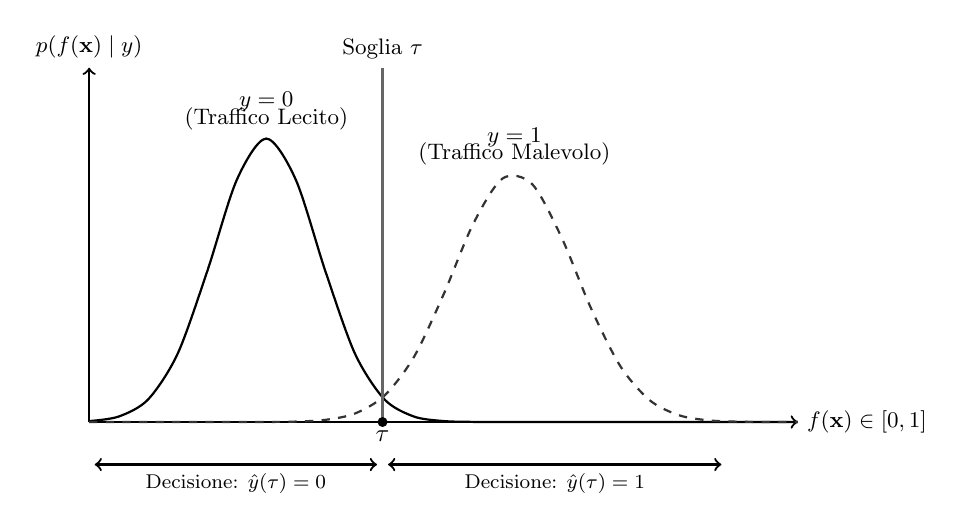
\begin{tikzpicture}[scale=0.9, every node/.style={transform shape}]
        % Assi cartesiani
        \draw[->, thick] (0,0) -- (10,0) node[right] {\small $f(\mathbf{x}) \in [0,1]$};
        \draw[->, thick] (0,0) -- (0,5) node[above] {\small $p(f(\mathbf{x}) \mid y)$};

        % Distribuzione Classe 0 (Lecito) - Linea continua
        \draw[thick, black, smooth, domain=0:10] plot (\x, {4.0*exp(-(\x-2.5)^2/1.1)});
        \node at (2.5, 4) [anchor=south, align=center] {
            \small $y=0$ \\[-5pt]
            \small (Traffico Lecito)
        };

        % Distribuzione Classe 1 (Malevolo) - Linea tratteggiata
        \draw[thick, dashed, black!80, smooth, domain=0:10] plot (\x, {3.5*exp(-(\x-6)^2/1.5)});
        \node at (6.0, 3.5) [anchor=south, align=center] {
            \small $y=1$ \\[-5pt]
            \small (Traffico Malevolo)
        };

        % Soglia decisionale tau
        \draw[very thick, gray!80!black] (4.14,0) -- (4.14,5);
        \node[above] at (4.14, 5) {\small Soglia $\tau$};
        \fill (4.14,0) circle (2pt) node[below] {$\tau$};

        % Regioni decisionali
        \draw[<->, thick, shorten >=2pt, shorten <=2pt] (0, -0.6) -- (4.14, -0.6) node[midway, below] {\footnotesize Decisione: $\hat{y}(\tau)=0$};
        \draw[<->, thick, shorten >=2pt, shorten <=2pt] (4.14, -0.6) -- (9, -0.6) node[midway, below] {\footnotesize Decisione: $\hat{y}(\tau)=1$};
    \end{tikzpicture}
    \caption{Mappatura della probabilità a posteriori $f(\mathbf{x})$ sulla regola decisionale binaria $\hat{y}(\tau)$ in funzione della soglia $\tau$.}
    \label{fig:soglia_decisionale}
\end{figure}

\subsubsection{Formalizzazione delle Metriche Derivate}
\label{subsubsec:metriche_derivate_formali}

Per rendere la valutazione indipendente dalla numerosità del campione di test, si introducono i principali tassi relativi derivati dalla matrice di confusione \cite{fawcett2006}:

\begin{equation}
    TPR(\tau)=\frac{TP(\tau)}{TP(\tau)+FN(\tau)},
    \qquad
    FPR(\tau)=\frac{FP(\tau)}{FP(\tau)+TN(\tau)}
\end{equation}

cui corrispondono i rispettivi complementari

\[
    FNR(\tau)=1-TPR(\tau),
    \qquad
    TNR(\tau)=1-FPR(\tau).
\]

L'affidabilità delle segnalazioni generate dal classificatore è invece misurata dalla \textit{Precision}:

\begin{equation}
    Precision(\tau)=\frac{TP(\tau)}{TP(\tau)+FP(\tau)}
\end{equation}

Per sintetizzare il compromesso tra capacità di rilevamento degli attacchi e contenimento dei falsi allarmi si utilizza l'\textit{F1-score}, definito come media armonica tra Precision e Recall\footnote{Nei sistemi NIDS la media armonica è preferita alla media aritmetica poiché penalizza maggiormente modelli caratterizzati da un forte sbilanciamento tra sensibilità agli attacchi e precisione delle segnalazioni.}:

\begin{equation}
    F_1(\tau)=2\cdot\frac{Precision(\tau)\cdot TPR(\tau)}{Precision(\tau)+TPR(\tau)}
\end{equation}

Infine, l'\textit{Accuracy} rappresenta la proporzione complessiva di classificazioni corrette:

\begin{equation}
    Accuracy(\tau)=\frac{TP(\tau)+TN(\tau)}{N}
\end{equation}

Tale indicatore assume tuttavia un ruolo secondario nei problemi di intrusion detection, poiché non risulta sufficientemente informativo in presenza di distribuzioni fortemente sbilanciate tra traffico nominale e traffico malevolo.

\subsubsection{Dinamica della Soglia e Analisi Grafica (ROC e PR AUC)}
\label{subsubsec:analisi_grafica}

La valutazione puntuale delle metriche presuppone la scelta di uno specifico valore della soglia decisionale (ad esempio $\tau=0.5$). Una caratterizzazione più completa del comportamento discriminativo del classificatore richiede invece l'analisi dell'intero intervallo di valori della soglia, $\tau\in[0,1]$.

A tale scopo si impiegano le curve \textit{Receiver Operating Characteristic} (ROC) e \textit{Precision--Recall} (PR), sintetizzate mediante l'area sottesa alla rispettiva curva (\textit{Area Under the Curve}, AUC):

\begin{equation}
    AUC_{ROC}=\int_{0}^{1}TPR\,d(FPR),
    \qquad
    AUC_{PR}=\int_{0}^{1}Precision\,d(TPR)
\end{equation}

\begin{figure}[H]
    \centering
    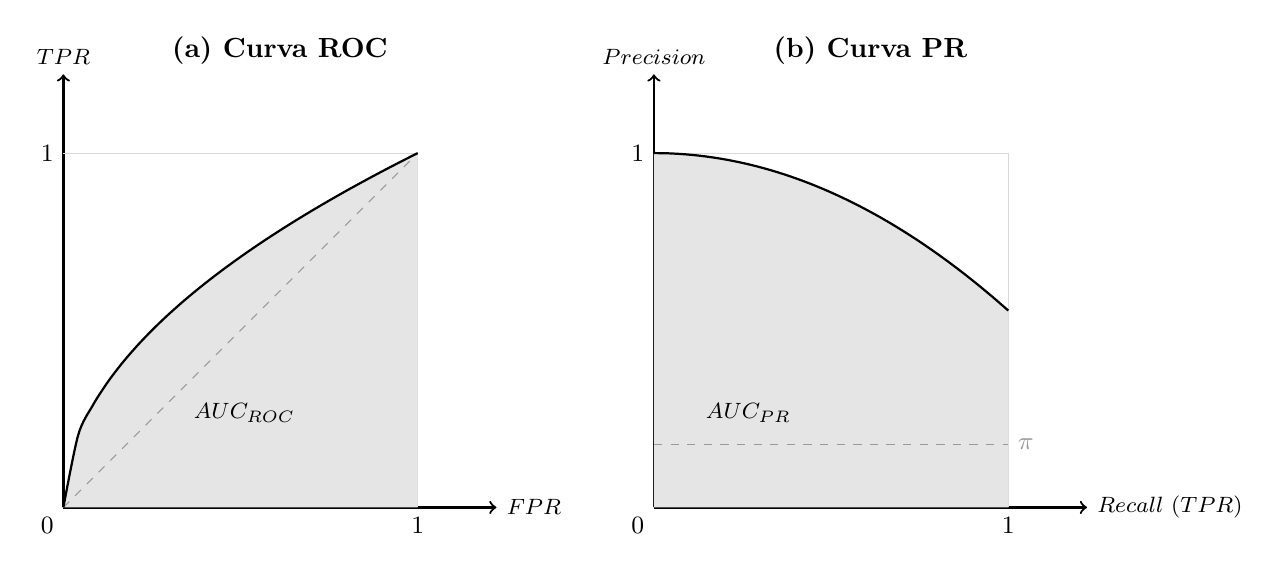
\begin{tikzpicture}
        % --- Sottofigura (a): Curva ROC ---
        \begin{scope}[shift={(0,0)}]
            % Assi
            \draw[->, thick] (0,0) -- (5.5,0) node[right] {\footnotesize $FPR$};
            \draw[->, thick] (0,0) -- (0,5.5) node[above] {\footnotesize $TPR$};

            % Griglia di riferimento
            \draw[gray!30, thin] (0,4.5) -- (4.5,4.5) -- (4.5,0);
            \node[below left] at (0,0) {\small $0$};
            \node[below] at (4.5,0) {\small $1$};
            \node[left] at (0,4.5) {\small $1$};

            % Area sottesa (AUC) in toni di grigio
            \fill[gray!20] (0,0) -- plot[smooth, domain=0:4.5] (\x, {4.5*sqrt(\x/4.5)}) -- (4.5,0) -- cycle;

            % Baseline casuale (diagonale)
            \draw[dashed, gray!80] (0,0) -- (4.5,4.5);

            % Curva ROC
            \draw[thick, black, smooth, domain=0:4.5] plot (\x, {4.5*sqrt(\x/4.5)});

            % Etichette
            \node at (2.3, 1.2) {\footnotesize $AUC_{ROC}$};
            \node[above] at (2.75, 5.5) {\textbf{(a) Curva ROC}};
        \end{scope}

        % --- Sottofigura (b): Curva Precision-Recall ---
        \begin{scope}[shift={(7.5,0)}]
            % Assi
            \draw[->, thick] (0,0) -- (5.5,0) node[right] {\footnotesize $Recall\ (TPR)$};
            \draw[->, thick] (0,0) -- (0,5.5) node[above] {\footnotesize $Precision$};

            % Griglia di riferimento
            \draw[gray!30, thin] (0,4.5) -- (4.5,4.5) -- (4.5,0);
            \node[below left] at (0,0) {\small $0$};
            \node[below] at (4.5,0) {\small $1$};
            \node[left] at (0,4.5) {\small $1$};

            % Area sottesa (AUC) in toni di grigio
            \fill[gray!20] (0,0) -- plot[smooth, domain=0:4.5] (\x, {4.5 - 2*(\x/4.5)^2}) -- (4.5,0) -- cycle;
            
            % Baseline prevalenza (linea orizzontale)
            \draw[dashed, gray!80] (0,0.8) -- (4.5,0.8) node[right] {\small $\pi$};

            % Curva PR
            \draw[thick, black, smooth, domain=0:4.5] plot (\x, {4.5 - 2*(\x/4.5)^2});

            % Etichette
            \node at (1.2, 1.2) {\footnotesize $AUC_{PR}$};
            \node[above] at (2.75, 5.5) {\textbf{(b) Curva PR}};
        \end{scope}
    \end{tikzpicture}
    \caption{Rappresentazione schematica dell'Area Sottesa alla Curva (AUC) per le analisi grafiche ROC (a) e Precision-Recall (b).}
    \label{fig:curve_roc_pr}
\end{figure}

L'indice $AUC_{ROC}$ fornisce una misura della capacità discriminativa complessiva del classificatore, mentre $AUC_{PR}$ risulta particolarmente indicato nei sistemi NIDS, dove la forte prevalenza del traffico legittimo rende più significativa la valutazione del compromesso tra Precision e Recall \cite{saito2015}.

\subsubsection{Degrado Prestazionale e Significatività Statistica (Welch's t-test)}
\label{subsubsec:significativita_statistica}

Il trasferimento di un modello tra domini caratterizzati da differenti distribuzioni marginali delle caratteristiche $P(\mathbf{x})$ (\textit{covariate shift}) può determinare una degradazione delle prestazioni di classificazione \cite{pan2010}. Tale variazione dell'efficacia discriminativa di un modello $M$, valutato sul dominio sorgente $\mathcal{D}_S$ e sul dominio target $\mathcal{D}_T$, può essere espressa come

\begin{equation}
    \Delta F_1=F_1(M,\mathcal{D}_S)-F_1(M,\mathcal{D}_T).
\end{equation}

Per valutare la significatività statistica delle differenze prestazionali tra modelli differenti, oppure tra un modello e una baseline di riferimento, si adotta il test $t$ di Welch, appropriato nel caso di campioni indipendenti con varianze non necessariamente uguali. Date due distribuzioni campionarie della metrica di interesse, caratterizzate da medie $\bar{x}_1$, $\bar{x}_2$, varianze $s_1^2$, $s_2^2$ e numerosità $n_1$, $n_2$, la statistica del test è definita da

\begin{equation}
    t=\frac{\bar{x}_1-\bar{x}_2}{\sqrt{\frac{s_1^2}{n_1}+\frac{s_2^2}{n_2}}}.
\end{equation}

I corrispondenti gradi di libertà effettivi sono stimati mediante l'approssimazione di Welch--Satterthwaite:

\begin{equation}
    \nu\approx\frac{\left(\frac{s_1^2}{n_1}+\frac{s_2^2}{n_2}\right)^2}{\frac{\left(s_1^2/n_1\right)^2}{n_1-1}+\frac{\left(s_2^2/n_2\right)^2}{n_2-1}}.
\end{equation}

L'ipotesi nulla di uguaglianza delle medie,

\[
    H_0:\mu_1=\mu_2,
\]

viene respinta qualora il valore $p$ associato alla statistica $t$ risulti inferiore al livello di significatività prefissato $\alpha$ (tipicamente $\alpha=0.05$), indicando che la differenza prestazionale osservata è statisticamente significativa e non può essere ragionevolmente attribuita al solo errore campionario.

\section[Sintesi del Capitolo e Raccordo con la Campagna Sperimentale]{Sintesi del Capitolo e Raccordo con la Campagna \\\ Sperimentale}
\label{sec:sintesi_raccordo_ch4}

L'impalcatura teorica e metodologica formalizzata nel presente capitolo definisce un modello astratto e rigoroso per la valutazione dei sistemi NIDS soggetti a \textit{domain shift}. 
Attraverso l'allineamento degli spazi delle \textit{feature}, la formalizzazione dei modelli di classificazione (aggregati e specialistici) e la definizione di un protocollo stocastico fondato su valutazioni \textit{multi-seed} e test di significatività, il framework garantisce l'isolamento dei reali contributi algoritmici dal rumore di misura.

Tuttavia, la validità dei vincoli analitici e delle proprietà di invarianza descritte richiede un riscontro quantitativo su scenari operativi concreti. 
Nel Capitolo~\ref{ch:risultati_sperimentali} \textcolor{red}{\textbf{[RICORDATI DI AGGIORNARE LA LABEL]}}, il framework teorico viene pertanto istanziato ed eseguito empiricamente. 
Verranno presentati la caratterizzazione dei dataset di traffico reale, il setup infrastrutturale di addestramento e la discussione critica dei risultati ottenuti, valutando le capacità di generalizzazione e le prestazioni dei modelli al variare dei contesti di rete.